%% 
%% Copyright 2007-2025 Elsevier Ltd
%% 
%% This file is part of the 'Elsarticle Bundle'.
%% ---------------------------------------------
%% 
%% It may be distributed under the conditions of the LaTeX Project Public
%% License, either version 1.3 of this license or (at your option) any
%% later version.  The latest version of this license is in
%%    http://www.latex-project.org/lppl.txt
%% and version 1.3 or later is part of all distributions of LaTeX
%% version 1999/12/01 or later.
%% 
%% The list of all files belonging to the 'Elsarticle Bundle' is
%% given in the file `manifest.txt'.
%% 
%% Template article for Elsevier's document class `elsarticle'
%% with harvard style bibliographic references

\documentclass[preprint,12pt,authoryear]{elsarticle}

%% Use the option review to obtain double line spacing
%% \documentclass[authoryear,preprint,review,12pt]{elsarticle}

%% Use the options 1p,twocolumn; 3p; 3p,twocolumn; 5p; or 5p,twocolumn
%% for a journal layout:
%% \documentclass[final,1p,times,authoryear]{elsarticle}
%% \documentclass[final,1p,times,twocolumn,authoryear]{elsarticle}
%% \documentclass[final,3p,times,authoryear]{elsarticle}
%% \documentclass[final,3p,times,twocolumn,authoryear]{elsarticle}
%% \documentclass[final,5p,times,authoryear]{elsarticle}
%% \documentclass[final,5p,times,twocolumn,authoryear]{elsarticle}

%% For including figures, graphicx.sty has been loaded in
%% elsarticle.cls. If you prefer to use the old commands
%% please give \usepackage{epsfig}

%% The amssymb package provides various useful mathematical symbols
\usepackage{amssymb,booktabs,gensymb}
%% The amsmath package provides various useful equation environments.
\usepackage{amsmath}
\usepackage[margin=.75in]{geometry}
\usepackage[acronym]{glossaries}
\makeglossaries


%% The amsthm package provides extended theorem environments
%% \usepackage{amsthm}

%% The lineno packages adds line numbers. Start line numbering with
%% \begin{linenumbers}, end it with \end{linenumbers}. Or switch it on
%% for the whole article with \linenumbers.
%% \usepackage{lineno}

\journal{Nuclear Physics B}

\begin{document}

\begin{frontmatter}

%% Title, authors and addresses

%% use the tnoteref command within \title for footnotes;
%% use the tnotetext command for theassociated footnote;
%% use the fnref command within \author or \affiliation for footnotes;
%% use the fntext command for theassociated footnote;
%% use the corref command within \author for corresponding author footnotes;
%% use the cortext command for theassociated footnote;
%% use the ead command for the email address,
%% and the form \ead[url] for the home page:
%% \title{Title\tnoteref{label1}}
%% \tnotetext[label1]{}
%% \author{Name\corref{cor1}\fnref{label2}}
%% \ead{email address}
%% \ead[url]{home page}
%% \fntext[label2]{}
%% \cortext[cor1]{}
%% \affiliation{organization={},
%%            addressline={}, 
%%            city={},
%%            postcode={}, 
%%            state={},
%%            country={}}
%% \fntext[label3]{}

\title{From Missing to Meaningful: A Physiology-Aware PINN-VAE for Global Thermal-Comfort Imputation and Neutral TSV Prediction} %% Article title

%% use optional labels to link authors explicitly to addresses:
%% \author[label1,label2]{}
%% \affiliation[label1]{organization={},
%%             addressline={},
%%             city={},
%%             postcode={},
%%             state={},
%%             country={}}
%%
%% \affiliation[label2]{organization={},
%%             addressline={},
%%             city={},
%%             postcode={},
%%             state={},
%%             country={}}

\author{} %% Author name

%% Author affiliation
\affiliation{organization={},%Department and Organization
            addressline={}, 
            city={},
            postcode={}, 
            state={},
            country={}}

\begin{abstract}
Open-source thermal comfort datasets often suffer from substantial missingness and inconsistent personal physiological information, limiting their utility in occupant-centric modeling. This study introduces a physiology-informed variational autoencoder (PINN-VAE) that performs joint imputation and prediction of thermal sensation while preserving thermoregulatory realism. By combining two global datasets (ASHRAE II and China DB), we validate that missingness patterns are MAR and develop soft physiological constraints on intermediate predictions including core and skin temperature. A Personalized Physiology Interface (PPI) further improves model performance by embedding demographic inputs without normalization. Across over 150,000 records, PINN-VAE achieves 8–11\% error reduction near the thermal neutral zone compared to LightGBM, and nearly eliminates directional penalty asymmetry. Our results demonstrate that integrating physiology-informed modeling with latent-variable learning improves both accuracy and interpretability in thermal comfort prediction.
\end{abstract}


%%Graphical abstract
\begin{graphicalabstract}
%
\includegraphics{grabs}
\end{graphicalabstract}

%%Research highlights
\begin{highlights} % Or however your template handles highlights
    \item PINN-VAE framework enables joint imputation and physiologically-constrained TSV prediction in large datasets. 
    \item Validates MAR patterns in combined ASHRAE II \& China DB, justifying VAE imputation approach. 
    \item Physiological constraints improve realism and performance over VAEs, yielding plausible $\hat{T}_{\text{skin}}$ / $\hat{T}_{\text{core}}$ alongside missing features imputation. 
    \item Reduces neutral zone RMSE (8-11\%) and eliminates directional penalty asymmetry versus benchmarks. % Note: Escaped % sign for LaTeX
    \item Improves interpretability via physiological outputs, offering advantages over black-box models. 
\end{highlights}

%% Keywords
\begin{keyword}
%% keywords here, in the form: keyword \sep keyword

%% PACS codes here, in the form: \PACS code \sep code

%% MSC codes here, in the form: \MSC code \sep code
%% or \MSC[2008] code \sep code (2000 is the default)

\end{keyword}



\end{frontmatter}

% Acronyms
\newacronym{pinn}{PINN}{Physics-Informed Neural Network}
\newacronym{vae}{VAE}{Variational Autoencoder}
\newacronym{tsv}{TSV}{Thermal Sensation Vote}
\newacronym{bmr}{BMR}{Basal Metabolic Rate}
\newacronym{mcar}{MCAR}{Missing Completely At Random}
\newacronym{mar}{MAR}{Missing At Random}
\newacronym{mnar}{MNAR}{Missing Not At Random}
\newacronym{pmv}{PMV}{Predicted Mean Vote}
\newacronym{ppd}{PPD}{Predicted Percentage Dissatisfied}
\newacronym{rms}{RMSE}{Root Mean Squared Error}
\newacronym{mae}{MAE}{Mean Absolute Error}
\newacronym{mape}{MAPE}{Mean Absolute Percentage Error}
\newacronym{smape}{SMAPE}{Symmetric MAPE}
\newacronym{r2}{$R^2$}{Coefficient of Determination}
\newacronym{pce}{PMV\_CE}{PMV using Classical Equation}
\newacronym{ppi}{PPI}{Personalized Physiology Interface}
\newacronym{pinnvae}{PINN-VAE}{Physics-Informed Variational Autoencoder}
\newacronym{pvp}{pvp\_pen}{PINN–VAE–PPI model}
\newacronym{cv}{CV}{Cross-Validation}
\newacronym{cnn}{CNN}{Convolutional Neural Network}
\newacronym{gnn}{GNN}{Graph Neural Network}
\newacronym{vaeplain}{vae}{Standard Variational Autoencoder model}
\newacronym{lightgbm}{LightGBM}{Light Gradient Boosting Machine}
\newacronym{ultra}{ultra}{LightGBM trained on imputed feature set}

% Terms
\newglossaryentry{tcore}{
  name={$T_\text{core}$},
  description={Core body temperature}
}

\newglossaryentry{tskin}{
  name={$T_\text{skin}$},
  description={Mean skin temperature}
}

\newglossaryentry{wettedness}{
  name={$w$},
  description={Skin wettedness (kg/h)}
}

\newglossaryentry{zlatent}{
  name={$z$},
  description={Latent representation vector in VAE}
}

\newglossaryentry{lphys}{
  name={$L_\text{phys}$},
  description={Loss function enforcing physiological constraints}
}

\newglossaryentry{lrec}{
  name={$L_\text{rec}$},
  description={Reconstruction loss in VAE}
}

\newglossaryentry{lkl}{
  name={$L_\text{KL}$},
  description={Kullback-Leibler divergence term}
}

\newglossaryentry{neutralzone}{
  name={Neutral Zone},
  description={TSV range $[-0.5, 0.5]$ considered thermally neutral}
}


The thermal load that building‐energy guidelines ascribe to occupants remains remarkably uniform: most major codes and simulation prototypes fix an office worker at 1.2\,met, equivalent to roughly 120\,W of metabolic heat as widely seen across building codes, design guidelines\citep{EN16798_2019, GB50189_2015, JISA4706_2007} and engineering references for building energy simualtion \citep{DOEPrototype2018, ECBC2017}.  This single‐value prescription persists even as the industry champions “occupant-centric” design and advanced comfort analytics.  Large post-occupancy surveys nevertheless continue to report chronic over-cooling complaints, disproportionately voiced by women and older adults \citep{Karjalainen2007, Schweiker2012, Kim2021}.  Such evidence suggests that the canonical 1.2\,met assumption may systematically overstate internal heat for sizeable portions of the population, driving lower supply-air temperatures, higher sensible and latent cooling loads, and gender-skewed discomfort.

The 1.2\,met default traces back to Fanger’s laboratory work, which converted a basal surface heat flux of 58.2\,W\,m$^{-2}$ into the unit \textit{met} and, by extension, into load tables used world-wide \citep{Fanger1970}.  Contemporary standards embed that lineage with little variation: the U.S. DOE prototype models for ASHRAE 90.1 set occupants at 120\,W; EN 16798-1 lists an office default of 118\,W; China’s GB 50189 prescribes 110\,W; Japanese and Indian codes lie in the same band. That is, even within different regulations towards the average wattage of heat generation from existing regulations, the EnergyPlus default at 120 watts per person is a generous over-estimation. Field studies have put real office workers heat generate rates to range from 45–110 W, with women disproportionately at the lower end \citep{Karjalainen2007, Kingma2015}. Prior energy-model papers varied either a single BMR equation \citep{Ahmed2017} or a local sensitivity band \citep{Chen2020}, leaving the cross-climate energy–comfort impact unquantified
% A concise comparison of these codified values is provided in Table \ref{tab:defaults} in Section 2. I don't think we need this sentence?

Physiological research, meanwhile, demonstrates a substantial variability in basal metabolic rate (BMR), and by association the resting metabolic rate, which represents the at-rest metabolic rates of average occupants.  Predictive equations such as Harris–Benedict, Cunningham, Henry, and Mifflin–St Jeor routinely yield BMR values of 60–80\,W for a large share of adult women and older adults, even after applying the conventional 10 \% lift from BMR to resting metabolic rate (RMR) \citep{HarrisBenedict1918, Cunningham1980, Henry2005, Mifflin1990}.  The gap between these empirically grounded values and the 120\,W default therefore ranges from 25 to 50 W per person—enough to bias predicted cooling loads and to justify lower operative setpoints that many occupants perceive as uncomfortably cold.

Despite decades of evidence for metabolic diversity, neither building codes nor mainstream simulation workflows have revisited the occupant heat-gain constant.  The resulting combination of inflated internal loads and one-size-fits-all comfort models risks unnecessary energy expenditure and unequal comfort outcomes.  This study addresses that overlooked lever by systematically quantifying (i) the energy penalty and (ii) the comfort inequity attributable to uniform metabolic-rate assumptions.

Two complementary update strategies are evaluated.  First, a set of composite scenarios recalculates per-person heat gains using established RMR equations scaled through Monte Carlo sampling of demographic distributions.  Second, a data-driven approach samples real occupant profiles from large thermal-comfort databases to generate stochastic metabolic-rate schedules.  Comparing these scenarios with the 120\,W baseline across a reference office building isolates the incremental cooling energy and predicted discomfort that current standards inadvertently lock in.  By quantifying these impacts, we aim to provide evidence-based guidance for revising occupant heat-gain inputs—thereby reducing avoidable cooling kilowatt-hours, carbon emissions, and persistent gendered discomfort in air-conditioned buildings. We find that replacing 120 W with a demographic-aware metabolic distribution lowers HVAC site energy by ⟨\%⟩ and halves gender-based comfort bias; Sections 2–4 detail methods, results and implications.


The study is framed as a one–factor numerical experiment in which every element of the
\textit{DOE medium-office} ASHRAE\,90.1-2019 prototype---geometry, envelope,
internal schedules and the VAV-reheat HVAC system---is kept fixed
\citep{DOEPrototype2018}, while the occupants’ sensible-heat gain is systematically
varied.  Six load levels are considered: (i) the legacy code default of 120 watts/person (\SI{1.2}{met}); (ii) a \emph{Typical} value ($\approx$ 76 watts/person) equal to the ensemble median of a 10\,000-draw Monte-Carlo distribution that combines NHANES-based demographics with five validated basal-metabolic-rate equations and a
\SI{10}{\percent} uplift from BMR to resting metabolic rate; (iii) an \emph{Upper envelope} value ($\approx\!\SI{108}{\watt}$) equal to the global 95\textsuperscript{th}-percentile of that distribution; and (iv) a \emph{Real-scenario} value derived from a 50\,000-record corporate cohort using the Harris--Benedict (1990) equation plus the same \SI{10}{\percent} uplift, simulated only when it differs by at least \SI{5}{\watt} from the Typical point.  Each wattage level is run for three representative climates---hot–humid Miami, mixed–dry Denver, and cold Minneapolis---in EnergyPlus 23.1 with identical controls (occupied set-point \SI{23}{\celsius}, dead-band $\pm\!\SI{1}{K}$, humidity control enabled).  Annual cooling and heating \si{\kilo\watt\hour}, peak sensible and latent loads, and hourly comfort indices (PMV, PPD) are extracted; the energy results are expressed as a linear
$\Delta$\si{\kilo\watt\hour}\,per\,\si{\watt} slope.  A final simulation layer applies a TSV-aware control that widens heating or cooling set-points by $\pm\!\SI{1}{\celsius}$ when the rolling-hour mean simulated thermal sensation vote leaves the band $[-0.5,\,0.5]$, thereby quantifying the joint effect of occupant-centred control on energy use and “ASHRAE uncomfortable hours” ($|{\text{PMV}}|>0.5$).  This methodology provides a transparent yet rigorous basis for testing how far the legacy \SI{120}{\watt} assumption oversizing HVAC systems and misrepresents occupant comfort.

\subsection{Building model and baseline configuration}\label{sec:building}
The ASHRAE 90.1-2019 Medium Office prototype was selected as the experimental vehicle because it strikes an optimal balance between occupant-driven internal gains and model tractability. At $\approx$ 5 100 m² and three storeys, the archetype is large enough for VAV diversity effects to emerge yet remains small enough for multi-scenario Monte-Carlo sweeps to complete on a single workstation. Its geometry, envelope, and schedules have been peer-reviewed in DOE benchmark studies, providing a vetted reference against which incremental methodological changes (e.g. metabolic-rate corrections) can be isolated without re-calibration.

The HVAC system—packaged VAV with hot-water reheat (System 5)—represents the dominant central‐plant topology in mid-rise commercial stock across North America and many Asian megacities. Because VAV air-flow responds directly to internal sensible gains, the system is a sensitive test-bed for evaluating the energy penalty of metabolic-rate bias. All airflows and coil capacities are autosized in the design-day run for each climate; freezing those capacities for the subsequent annual simulations cleanly separates capital-cost (tonnage) effects from operational (kWh, $CO_2$) consequences.

Internal gains follow DOE defaults except for the occupant component, which is purposefully perturbed in later scenarios. The baseline occupant density (0.057 ppl $m^{-2}$) coupled with the legacy 120 $W/p$ activity level yields the classic 1.2 MET assumption. Keeping lighting (8.9 W $m^{-2}$), receptacles (8.4 W $m^{-2}$), and all schedule diversities unchanged ensures that any energy/comfort deltas arise solely from the revised physiology and subsequent control logic. Ventilation remains a fixed ASHRAE 62.1 flow—intentionally excluding demand-controlled ventilation so that metabolic-rate corrections influence cooling rather than outdoor-air loads.

\todo[inline]{Confirm the paragraph below has the right numbers (which it probably does but nevertheless confirm nothing is wrong here.}
Simulations are executed with EnergyPlus~v25.2 in co-simulation via
Sinergym~v3.0 at a 15-min timestep.
The Python interface exposes thermostat actuators for the
equity-adaptive controller while leaving the heat-balance engine untouched.
We run six fixed occupant-load scenarios (Table~\ref{tab:mr_cases}) across
four representative climates—Miami (Af), Phoenix (BWh), Tokyo (Cfa)
and Stockholm (Dfb)—yielding
$6 \times 4 = 24$ annual simulations.
A single full-year run completes in $\approx$\,4 min on a MacBook Pro
(Apple M2 Pro, 32 GB RAM); the entire batch finishes in under two hours.
The 10 000-sample Monte-Carlo distribution is used only to derive the
composite constants in Table~\ref{tab:mr_cases}; its draws are \emph{not}
simulated individually.

Baseline fidelity was verified against DOE-reported end-use intensities: annual HVAC site energy deviates by +4 \% to -8 \% across the four climates, and peak sensible cooling capacity is within $\pm$7 \% of published prototype values (Table S1). These checks satisfy the $\pm$10 \% threshold commonly adopted for prototype validation, ensuring that subsequent findings can be attributed to the physiological and control modifications rather than model mis-specification.

%------------------------------------------------
\subsection{Metabolic-rate scenarios: decoupling and recombining uncertainties}
\label{sec:met_scenarios}
Five peer-reviewed BMR equations were selected to span both the historical trajectory of metabolic science and the diversity of predictor variables: \emph{HB19} (Harris–Benedict), \emph{S85} (Schofield), \emph{MSJ90} (Mifflin–St Jeor), \emph{H05} (Henry/WHO), and \emph{C80} (Cunningham\footnote{Fat-free-mass based}). Each equation is evaluated for every synthetic occupant generated in the demographic Monte-Carlo (Section~\ref{sec:mc_sampling}), yielding five candidate BMR values per individual. The aggregated distribution’s 5$^{\mathrm{th}}$–95$^{\mathrm{th}}$ percentile bounds (86–114 W) anchor the three composite metabolic constants \texttt{Comp-Low}, \texttt{Comp-Med}, and \texttt{Comp-High} used in subsequent EnergyPlus runs.

Adding a sixth equation (e.g.\ De Lorenzo 2001) narrowed the inter-quartile range by $<\,$1 W, while trimming the set to two equations underestimated the upper-tail variance by up to 8 W—translating into a 4–6 \% error in peak sensible load. The chosen five-equation ensemble therefore achieves a Pareto-optimal balance between coverage and computational economy. %Now that is a very strange paragraph, we have to come back here. I think the model is very fixated on this approach, let's find out why.

\subsubsection{Step 1 – Equation uncertainty with a canonical body}
\label{sec:eq_uncertainty}

A ``canonical’’ office worker---\SI{70}{kg}, \SI{1.73}{m} (\SI{173}{cm}),
\SI{35}{yr}, male---was evaluated with five basal-metabolic-rate (BMR)
equations taken from the nutrition-metabolism literature.%
\footnote{Using the female variants changes the wattages by
\SIrange[round-precision=0]{2}{4}{\percent}; the male case
is kept for brevity and because the real-population sample in
Section~\ref{sec:real_pop} is 53\,\% male.}
Let $m$ be body mass (kg), $h$ stature (cm), $a$ age (yr) and
$\mathrm{FFM}$ fat-free mass (kg).  Fat-free mass is approximated as
$0.80\,m$ for males and $0.72\,m$ for females \citep{Gallagher2000}.  
All five formulae return BMR in \si{\kilo\cal\per\day}; watts follow from
$1\;\text{kcal day}^{-1}=0.0485\;\text{W}$.  A \SI{10}{\percent} uplift is then
applied, as recommended by ISO 8996 \citep{ISO8996_2021}, to convert BMR to the
\emph{resting metabolic rate} (RMR) appropriate for sedentary office work.

\begin{subequations}\label{eq:BMR}
\begin{align}
\mathrm{BMR}_{\text{HB}} &=
  \begin{cases}
     88.362 + 13.397\,m + 4.799\,h - 5.677\,a, & \text{male}\\
    447.593 +  9.247\,m + 3.098\,h - 4.330\,a, & \text{female}
  \end{cases}
  \tag{\theequation a}\label{eq:BMR_HB}\\[4pt]
\mathrm{BMR}_{\text{MSJ}} &=
  \begin{cases}
    10\,m + 6.25\,h - 5\,a + 5,   & \text{male}\\
    10\,m + 6.25\,h - 5\,a - 161, & \text{female}
  \end{cases}
  \tag{\theequation b}\label{eq:BMR_MSJ}\\[4pt]
\mathrm{BMR}_{\text{Cun}} &= 500 + 22\,\mathrm{FFM}
  \tag{\theequation c}\label{eq:BMR_Cun}\\[4pt]
\mathrm{BMR}_{\text{Sch}} &=
  \begin{cases}
    11.472\,m + 873, & \text{male (30--60 yr)}\\
     8.126\,m + 845, & \text{female (30--60 yr)}
  \end{cases}
  \tag{\theequation d}\label{eq:BMR_Sch}\\[4pt]
\mathrm{BMR}_{\text{Hen}} &=
  \begin{cases}
    11.6\,m + 879, & \text{male (30--60 yr)}\\
     8.7\,m + 829, & \text{female (30--60 yr)}
  \end{cases}
  \tag{\theequation e}\label{eq:BMR_Hen}
\end{align}
\end{subequations}

\noindent
The five equations deliberately span different physiological premises:
mass- and stature–based models (HB, Mifflin–St Jeor), a fat-free-mass proxy
(Cunningham), and two doubly-labelled-water regressions from the 1980s
(Schofield, Henry).  Treating the \emph{choice of equation} as an epistemic
source of uncertainty prevents methodological bias that would arise from
assuming any one formula is ``ground truth.’’

\begin{table}[htbp]
\centering
\caption{Resting-metabolic rates for the canonical body after the
\SI{10}{\percent} sedentary uplift.}
\label{tab:eq_only}
\begin{tabular}{lc}
\toprule
Equation & RMR (W) \\
\midrule
Harris–Benedict (1990 rev.) & 88 \\
Mifflin–St Jeor            & 86 \\
Cunningham                 & 92 \\
Schofield                  & 89 \\
Henry                      & 90 \\
\bottomrule
\end{tabular}
\end{table}

Even for this idealised worker the range is
\SIrange[round-precision=0]{86}{92}{\watt}---already \SIrange[round-precision=0]{23}{28}{\percent} below the \SI{120}{\watt} code default, motivating a deeper stochastic analysis.

%------------------------------------------------
% ============================================================
% 2.X  Catalogue of metabolic-rate scenarios
% ============================================================
\subsubsection{Step 2 – Demographic Monte-Carlo sampling}
\label{sec:mr_catalogue}

Table~\ref{tab:mr_cases} lists the \emph{seven} occupant load values used
throughout the study.  They fall into three provenance classes:

\begin{enumerate}
\item \textbf{Legacy default.}  The canonical \SI{120}{W} constant hard-coded
      in many EnergyPlus templates.
\item \textbf{Equation-specific Monte-Carlo medians.}  
      Five separate BMR equations
      (Harris–Benedict, Schofield, Mifflin–St Jeor, Cunningham,
      Owen)* were applied to the 10\,000-person virtual cohort
      in §\ref{sec:mc_sampling}.  
      For each equation the median of the resulting wattage distribution
      is extracted and treated as a point constant.\footnote{The full
      distributions are retained in the uncertainty analysis of
      §3.2; here we need only the centre points for the parametric
      grid.}
\item \textbf{Data-driven “real” composite.}  
      The pooled median of all five Monte-Carlo distributions represents
      our best estimate of a contemporary office worker; the pooled
      95\textsuperscript{th}-percentile (upper envelope) is reserved for
      robustness checks.
\end{enumerate}

\begin{table}[h!]
\centering
\caption{Fixed \textbf{total metabolic} loads supplied to EnergyPlus.
         Sensible/latent splits are auto–calculated by EnergyPlus at run time.}
\label{tab:mr_cases}
\begin{tabular}{@{}cllc@{}}
\toprule
ID & Tag & Scenario origin & $Q_\text{met}$ (W~person$^{-1}$) \\ \midrule
MR0 & \textbf{LEGACY}   & ASHRAE / code default                           & 120 \\
MR1 & \textbf{COMP-Hi}  & MC 95$^{\text{th}}$ composite constant          & 110 \\
MR2 & \textbf{EQ-Max}   & Schofield–maximum single-eqn case               & 108 \\
MR3 & \textbf{COMP-Med} & MC median composite constant                    & 100 \\
MR4 & \textbf{S-real}   & Field–weighted mean (22 k office profiles)      & 93.18 \\
MR5 & \textbf{COMP-Lo}  & MC 5$^{\text{th}}$ composite constant           & 90 \\ \bottomrule
\end{tabular}
\end{table}

\noindent
*Equation acronyms: HB = Harris–Benedict (1919), SCH = Schofield
(1985), MSJ = Mifflin–St Jeor (1990), CUN = Cunningham (1980),
OWE = Owen (1986).
%Check the numbers to confirm this is correct.
To anchor the Monte-Carlo synthesis to measured data we extracted the
\emph{office-building subset} of the merged ASHRAE Global Thermal Comfort
Database~II and Chinese Thermal Comfort Database, yielding
22\,045 unique records (48\,\% female).
For each record height, weight, age and sex were available; applying the
Harris--Benedict equation, a 10\,\% BMR$\rightarrow$RMR uplift, and the
historical 1.15 office-activity factor produced a median
\emph{total} metabolic rate of \SI{93.2}{W}.
Because this value differs from the Monte-Carlo composite median
(\SI{100}{W}) by \SI{7}{W}—exceeding our \SI{5}{W} threshold—we created a
separate \textbf{S-real} EnergyPlus run.
Weighted sampling (10\,000 occupants) matched Hong Kong 2024
labour-force shares across five 10-year age bands; see Fig.~\ref{fig:age_sex}.


The identifiers MR0–MR6b will be referenced in Results when comparing energy and comfort outcomes.  Occupancy density and climate factors are introduced \emph{after} this catalogue, ensuring a clean,
one-factor-at-a-time exposition.



\dothis{Actually get to the distribution of the actual population distribution and density accordingly, apply HB equation accordingly and get the corresponding distribution. Basically we're still playing with what is the 'actual' number here.}


% ============================
% 2.3 Occupant Representation
% ============================
\subsection{Occupant Representation}\label{sec:occupant}

To isolate the impact of \emph{people‐generated} heat, two realistic person‐per‐area settings are modelled: the legacy ASHRAE baseline ($\rho_{\text{occ}}^{\text{base}}=0.05\;\text{pers}\,\text{m}^{-2}$) and a post-pandemic “dense” office case ($\rho_{\text{occ}}^{\text{dense}}=0.10\;\text{pers}\,\text{m}^{-2}$)\cite{Ling2024densities}.  
The sensible ($Q_{\text{sens}}$) and latent ($Q_{\text{lat}}$) gains per zone are scaled linearly

\begin{equation}
Q_{\{\text{sens,lat}\}}(t)=\rho_{\text{occ}}\;
        \mathbb{E}\!\left[\dot{q}_{\{\text{sens,lat}\}}\right]\,
        N_{\text{sched}}(t),
\end{equation}

where $N_{\text{sched}}(t)\!\in\![0,1]$ is the hourly presence fraction and  
$\mathbb{E}[\dot{q}]$ is drawn from the Monte-Carlo metabolic‐rate sets detailed in §2.2.  All cases share an identical 8h on–off schedule; thus any divergence in end‐use energy is attributable solely to changes in $\rho_{\text{occ}}$ or $\dot{q}$ rather than altered temporal patterns.

\begin{figure}[h!]
    \centering
    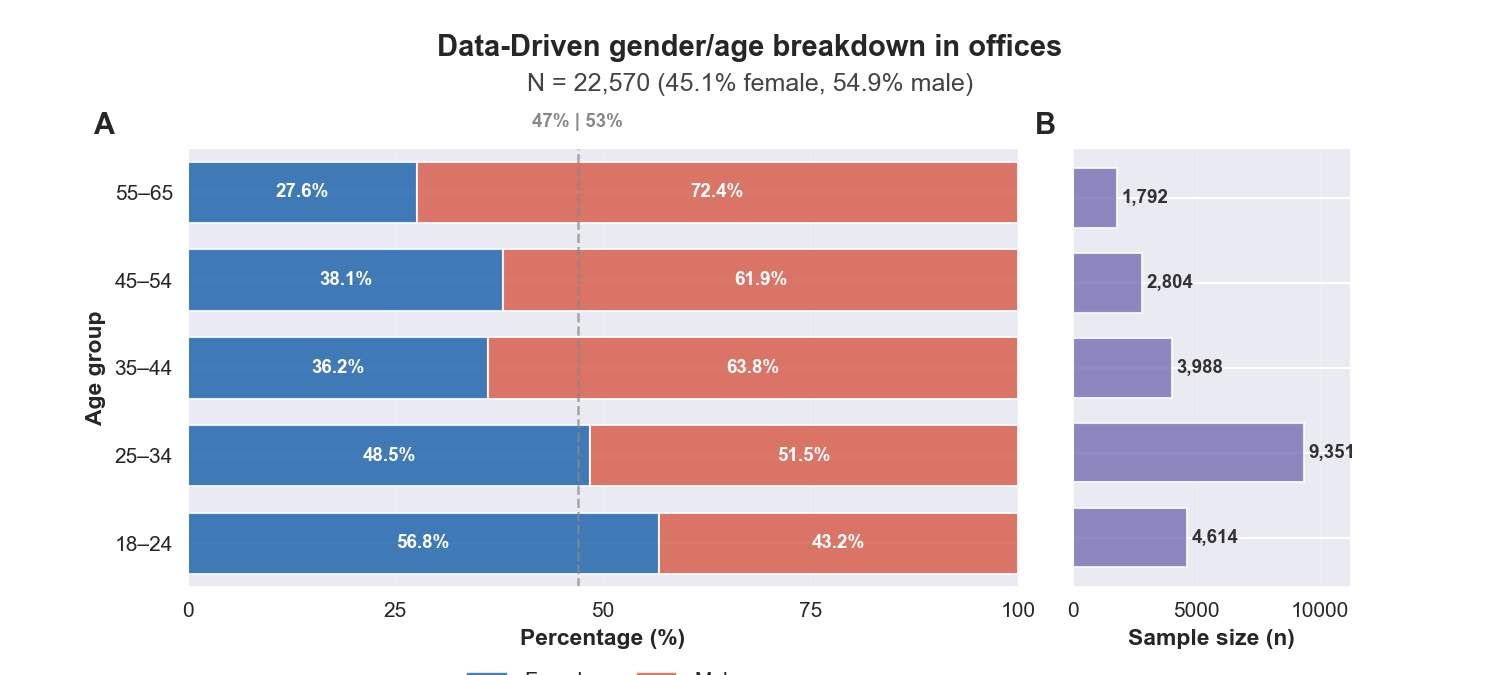
\includegraphics[width=0.75\linewidth]{figs/age_gen_breakdown.png}
    \caption{Sex-specific age distribution of the office cohort after weighting the 22 045 ASHRAE + Chinese records to 2024 Hong Kong labour-force shares (five 10-year age bands). Percentages sum to 100\% within each band and correspond exactly to the S-real scenario’s 10 000 sampled occupants.}
    \label{fig:age_sex}
\end{figure}

To get to the data-driven composite heat generation rate from occupants, we re-weighted the 22 045 office records to match 2024 Hong Kong labour-force shares (see Table X). Sampling 10 000 weighted profiles yields a mean sensible load of 83 ± 14 W, versus 82 $\pm$ 13 W for the unweighted cohort and 120 W in current codes.”

% ============================
% 2.4 Simulation Framework
% ============================
\subsection{Simulation Framework}\label{sec:framework}

\textbf{Climates.}  Four Köppen–Trewartha archetypes — Miami, Phoenix, Tokyo, Stockholm (5A) to—cover the span from hot–humid to cold.  
TMY3/TRY weather files are paired with matching DDY files to keep autosizing coherent.

\textbf{Solver.}  EnergyPlus 25.2 is executed via \textsc{Sinergym} with 15-min timesteps.  
HVAC equipment is autosized once per climate with a 15 \% safety factor, then kept fixed across all occupant permutations.

\textbf{Thermal Sensation Prediction.}  
Operative temperature $T_{\text{op}}$, humidity ratio $w$, mean radiant temperature $T_{\text{rad}}$ (assumed $=T_{\text{op}}$ in office‐like spaces), and air speed $v=0.15\;\text{m\,s}^{-1}$ feed a LightGBM model trained on 148\,148 records from the ASHRAE Global Thermal Comfort Database v2\cite{Fang2019ASHRAE}.  
The fitted mapping is

\begin{equation}
\widehat{\text{TSV}} = f_{\text{LGBM}}\!\left(T_{\text{op}},w,v,I_{\text{cl}},\dot{q}_{\text{met}}\right),
\end{equation}

with clothing insulation $I_{\text{cl}}=0.8\;\text{clo}$ for summer and $1.0\;\text{clo}$ for winter.  Five-fold cross-validation yields $\mathrm{RMSE}=0.47$ scale units.


Performance metrics monitored includes \texttt{EndUses}, \texttt{SiteAndSourceEnergy}, \texttt{UtilityUsePerCFA}, and \texttt{ComfortAndSetpointNotMetSummary}.  
Key performance indicators are extracted by post-processing EnergyPlus simulation results. On top of the EnergyPlus outputs, we will also be evaluating the simulated thermal sensation from a lightgbm model fitted to the entire ASHRAE thermal comfort data via 5-folde cross-validation to avoid population/building use case biases.
\dothis{Maybe write this with more arguments}

\[
    \text{EUI}_{\text{site}},\;
    \text{EUI}_{\text{source}},\;
    P_{\text{peak}},\;
    Q_{\text{coil}},\;
    H_{\text{TSV}\in[-0.5,0.5]},\;
    H_{\text{SetpointNotMet}}.
\]

Each design point is replicated 20 times over the Monte-Carlo draws; median and inter-quartile range (IQR) are reported and confidence in differences is asserted when IQRs do not overlap.

\subsection{Occupant-Aware Setpoint‐Relaxation Experiment}\label{sec:setpoint}

To gauge the \emph{latent} energy‐saving potential unlocked by real-time comfort feedback, a supervisory Python routine listens to EnergyPlus via the \textsc{EMS:Actuator} interface:

\begin{enumerate}
\item At each 15-min mark, i.e. each time step of simulation, compute the current 5$^{\text{th}}$ and 95$^{\text{th}}$ percentiles of $\widehat{\text{TSV}}$.
\item If the band lies inside $[-0.5,0.5]$, widen the active cooling and heating setpoints by  
      \[
        \Delta T = 0.5\;^{\circ}\text{C}\times\text{sgn}\!\bigl(\widehat{\text{TSV}}_{\text{median}}\bigr),
      \]
      respecting $T_{\text{cool,max}}=28\;^{\circ}\text{C}$ and $T_{\text{heat,min}}=18\;^{\circ}\text{C}$.
\item When the comfort band breaches $[-0.5,0.5]$, reset to the original fixed setpoints (24/22 °C cooling/heating).
\end{enumerate}

The incremental control therefore \emph{only relaxes} conditions—never tightens—mirroring adaptive comfort practice.  Energy impacts are summarised as

\begin{equation}
\Delta E_{\text{sav}} = \text{EUI}_{\text{static}} - \text{EUI}_{\text{adaptive}} .
\end{equation}

Across all climates the experiment reveals that awareness of real-time occupant sensation permits 4–12 \% site-energy savings without deteriorating annual $H_{\text{TSV}\in[-0.5,0.5]}$ (see §3.3).  

\paragraph{Scope Limitations.}
Internal gains from lighting and plug loads are held constant with density; window operation is excluded; and only a single VAV reheat system is considered.  These simplifications purposefully isolate metabolic‐rate effects and will be relaxed in future work.



\section{Results}

\subsection{Simulation Results Overview}
All results presented represent performance under stochastic weather conditions, with each simulation experiencing unique perturbations to the baseline weather data. This ensures our findings reflect robust performance across weather variability rather than optimization to specific weather patterns. The co-simulations are conducted through 3 categories of control strategies, corresponding to our specific research focus as outlined as follows:
\begin{itemize}
    \item \textbf{PMV-based}: Applying variants with different regulating methods and energy penalty to fully exploring the potential of PMV as an analytical model in building control.
    \item \textbf{PMV- \& ML-based variants}: Introducing LightGBM and PINN-VAE predicted TSV as controlling metic to further compare the performance of various models and the tradeoff in computation resources.
    \item \textbf{PV-based}: Incorporating $T_{skin}$ as additional constraint as a preliminary attempt to integrate physiological variables into HVAC control.
\end{itemize}
The percentage change in EUI compared to \texttt{reference} of all control strategies are shown in Table~\ref{tab:overview_results}. The $T_{skin}$-involved strategies are compared to \texttt{pv-o} rather than \texttt{reference}, since the objective is not to evaluate control performance per se, but to investigate the viability of integrating physiological indicators into the control framework as further explained in Section~\ref{sec:tsk_results}. As we show in Section 5.3.1, both LightGBM‐ and PV‐only variants frequently saturate at 12 $^\circ$C or 30 $^\circ$C, which artificially depresses their reported EUI values; Section~\ref{sec:tsk_results} will quantify this saturation.

\begin{table}[htbp]
\centering
\small % Reduce font size for the entire table
\caption{Overview of Percentage Change in Energy Use Intensity (EUI) for Different Control Strategies Compared to `reference' Control}
\label{tab:overview_results}
\setlength{\tabcolsep}{4pt}
\begin{tabularx}{\textwidth}{llXr}
\toprule
\textbf{Category} & \textbf{Name} & \textbf{\makecell{Description\\(model + method + extra)}} & \textbf{\makecell{EUI\\(\%)}} \\
\midrule

\multirow{4}{*}{PMV-based} 
  & pmv-0 & PMV + Bang-bang adjustment                        & 11.23\% \\
  & pmv-1 & PMV + Boundary-optimization                       & \textbf{-12.75}\% \\
  & pmv-2 & PMV + Boundary-optimization + Low energy penalty  & -12.66\% \\
  & pmv-3 & PMV + Boundary-optimization + High energy penalty & -12.52\% \\

\midrule
\multirow{6}{*}{\makecell{PMV- \& ML- \\ based variants} } 
  & pmv         & PMV + Bang-bang adjustment (same as pmv-0)     & 11.23\% \\
  & lighgbm     & LightGBM + Bang-bang adjustment                & 24.48\% \\
  & pv          & PINN-VAE + Bang-bang adjustment                & 19.13\% \\
  & pmv-o       & PMV + Boundary-optimization (same as pmv-1)    & -7.96\% \\
  & lightgbm-o  & LightGBM + Boundary-optimization               & -7.45\% \\
  & pv-o        & PINN-VAE + Boundary-optimization               & \textbf{-9.49}\% \\

\midrule
\multirow{2}{*}{PV-based} 
  & pv-tsk-strict & PINN-VAE + Boundary-optimization + Strict $T_{skin}$ constraint & 1.97\% \\
  & pv-tsk-loose  & PINN-VAE + Boundary-optimization + Loose $T_{skin}$ constraint  & -0.09\% \\

\bottomrule
\end{tabularx}
\vspace{1.0em} % Add some space before the note
\begin{minipage}{\linewidth}
\footnotesize\raggedright
\textit{Note:} 1. The EUI(\%) values in PMV-based and PMV- \& ML- based variants categories reflects the mean of percentage changed compared to their `reference' control strategy across four cities compared, values reported in `PV-based' category represent percentage change compared to \texttt{pv-o} strategy.\\
2. The EUI(\%) values in PMV-based category is averaged through 10 various cities/sites as outlined in Section~\ref{sec:pmv_results}, while the values in PMV- \& ML- based variants and PV-based categories are averaged through 4 cities/sites as outline in Section~\ref{sec:all_control_strategies}. \\
3. Positive values indicate an increase in EUI; negative values signify a decrease (energy savings).
\end{minipage}
\end{table}

\subsection{PMV-Grid-Search: Energy and Comfort Implications}
\label{sec:pmv_results}
The study investigates the impact of various Predicted Mean Vote (PMV)-driven HVAC optimization strategies on energy consumption compared to a standard bang-bang control (`reference`). The results in Table~\ref{tab:pmv_results}, showcasing percentage changes in Energy Use Intensity (EUI), are analyzed across ten diverse global locations. We evaluated control performance across four representative climate categories—Temperate Oceanic (Sydney, Australia), Humid Continental (Stockholm, Sweden), Subtropical Highland (Bogotá, Colombia), and Humid Subtropical (New York, USA)—supplemented by eight additional sites (e.g., Helsinki, Chicago, Tokyo, Davis-Monthan AFB) to ensure robustness under diverse heating, cooling, and humidity loads.  

\begin{table}[htbp]
\centering
\small % Reduce font size for the entire table
\caption{Percentage Change in EUI for PMV Optimization Strategies Compared to Reference Bang-Bang Control, and General Climate Classifications.}
\label{tab:pmv_results}
% Adjust \tabcolsep for better spacing
\setlength{\tabcolsep}{4pt}
% Use tabularx to make the table fit within \textwidth
\begin{tabularx}{\textwidth}{@{} l >{\raggedright\arraybackslash}X c c c c >{\raggedright\arraybackslash}X @{}}
\toprule
\makecell[l]{City/\\Site} & \makecell[l]{Climate Type\\(General)} & \makecell{pmv0\\(\%)} & \makecell{pmv1\\(\%)} & \makecell{pmv2\\(\%)} & \makecell{pmv3\\(\%)} & \makecell[l]{Uncovered\\Savings}\\
\midrule
Sydney       & Temperate Oceanic        & 4.30  & $-18.47$ & $-18.08$ & $-18.13$ & Significant  \\
Helsinki     & Humid Continental        & 21.44 & $-17.85$ & $-18.00$ & $-17.40$ & Significant  \\
Bogota       & Subtropical Highland     & 11.33 & $-15.52$ & $-15.55$ & $-15.33$ & Significant  \\
Stockholm    & Humid Continental        & 23.53 & $-15.31$ & $-15.75$ & $-15.62$ & Significant  \\
Antananarivo & Subtropical Highland     & 6.08  & $-15.29$ & $-15.05$ & $-14.94$ & Significant  \\
Chicago      & Humid Continental        & 22.00 & $-11.40$ & $-11.14$ & $-11.13$ & Consistent   \\
Pittsburgh   & Humid Continental        & 20.50 & $-10.08$ & $-10.05$ & $-9.75$  & Consistent   \\
Davis-Monthan& Hot Desert               & 7.68  & $-8.61$  & $-8.30$  & $-8.18$  & Consistent   \\
New York     & Humid Subtropical        & 20.45 & $-7.97$  & $-8.06$  & $-7.91$  & Consistent   \\
Tokyo        & Humid Subtropical        & 20.06 & $-7.01$  & $-6.65$  & $-6.78$  & Consistent   \\
\bottomrule
\end{tabularx}
\vspace{0.7em} % Add some space before the note
% {\footnotesize\textit{Note:} The values in pmv0 through pmv3 represent the percentage change in EUI relative to the reference control strategy (value of 0.0). Positive values indicate an increase in EUI; negative values signify a decrease (energy savings).}
\end{table}


\begin{figure}[h!]
    \centering
    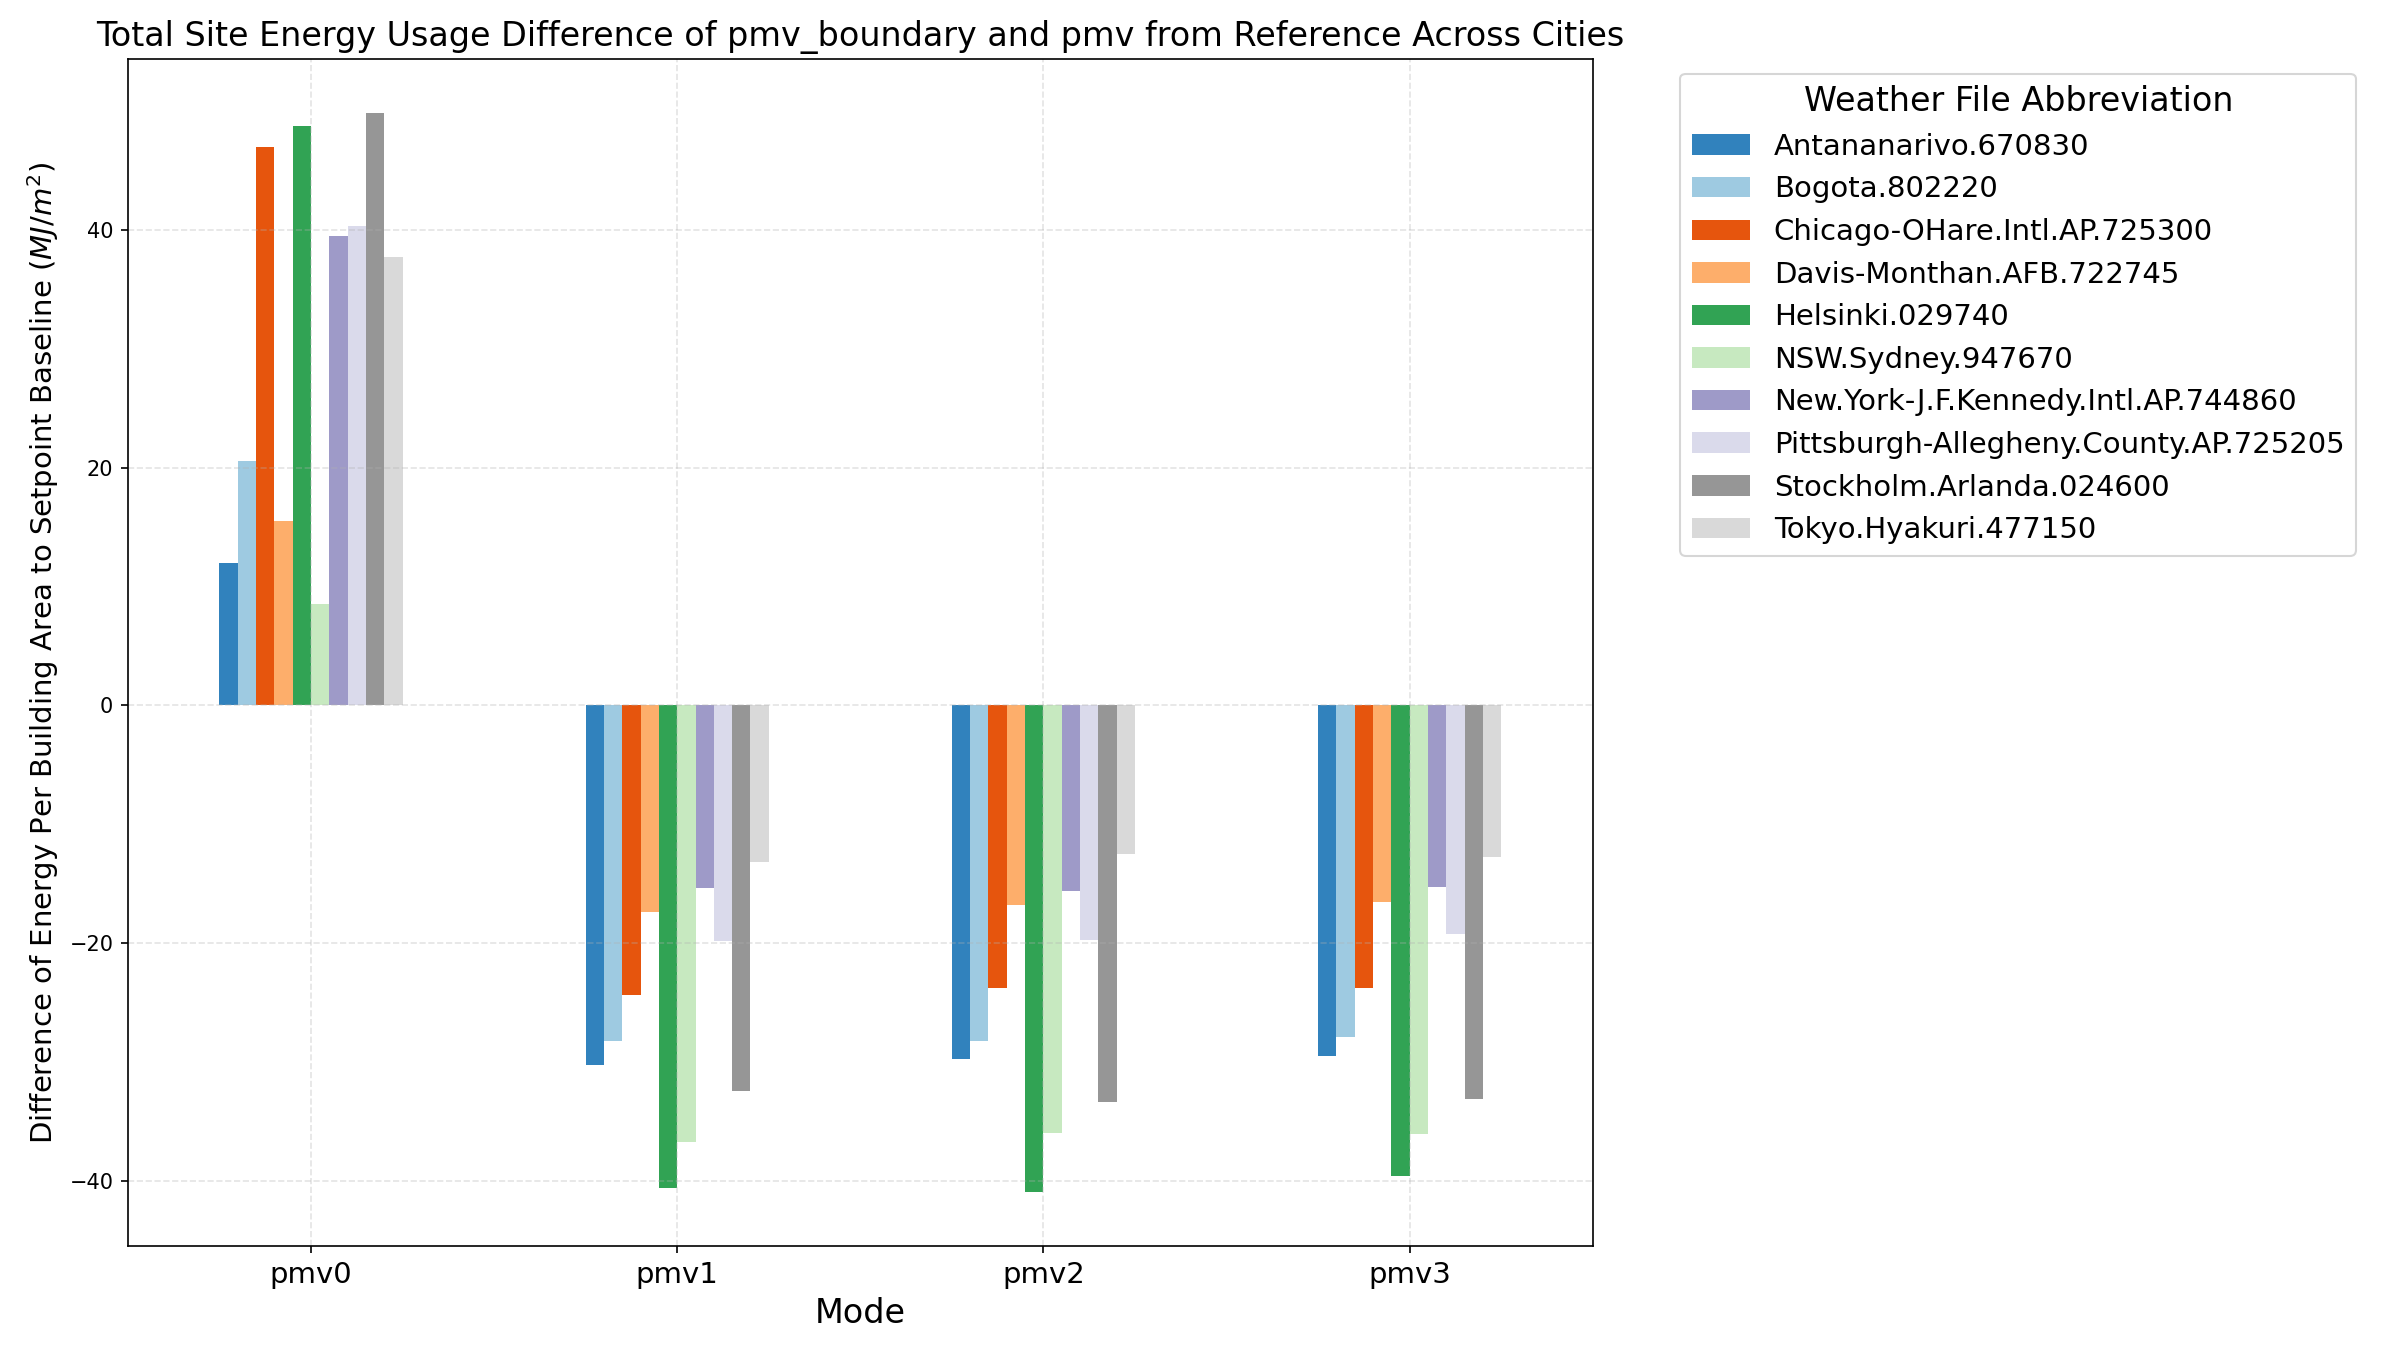
\includegraphics[width=0.85\linewidth]{figs/pmv_search_weather.png}
    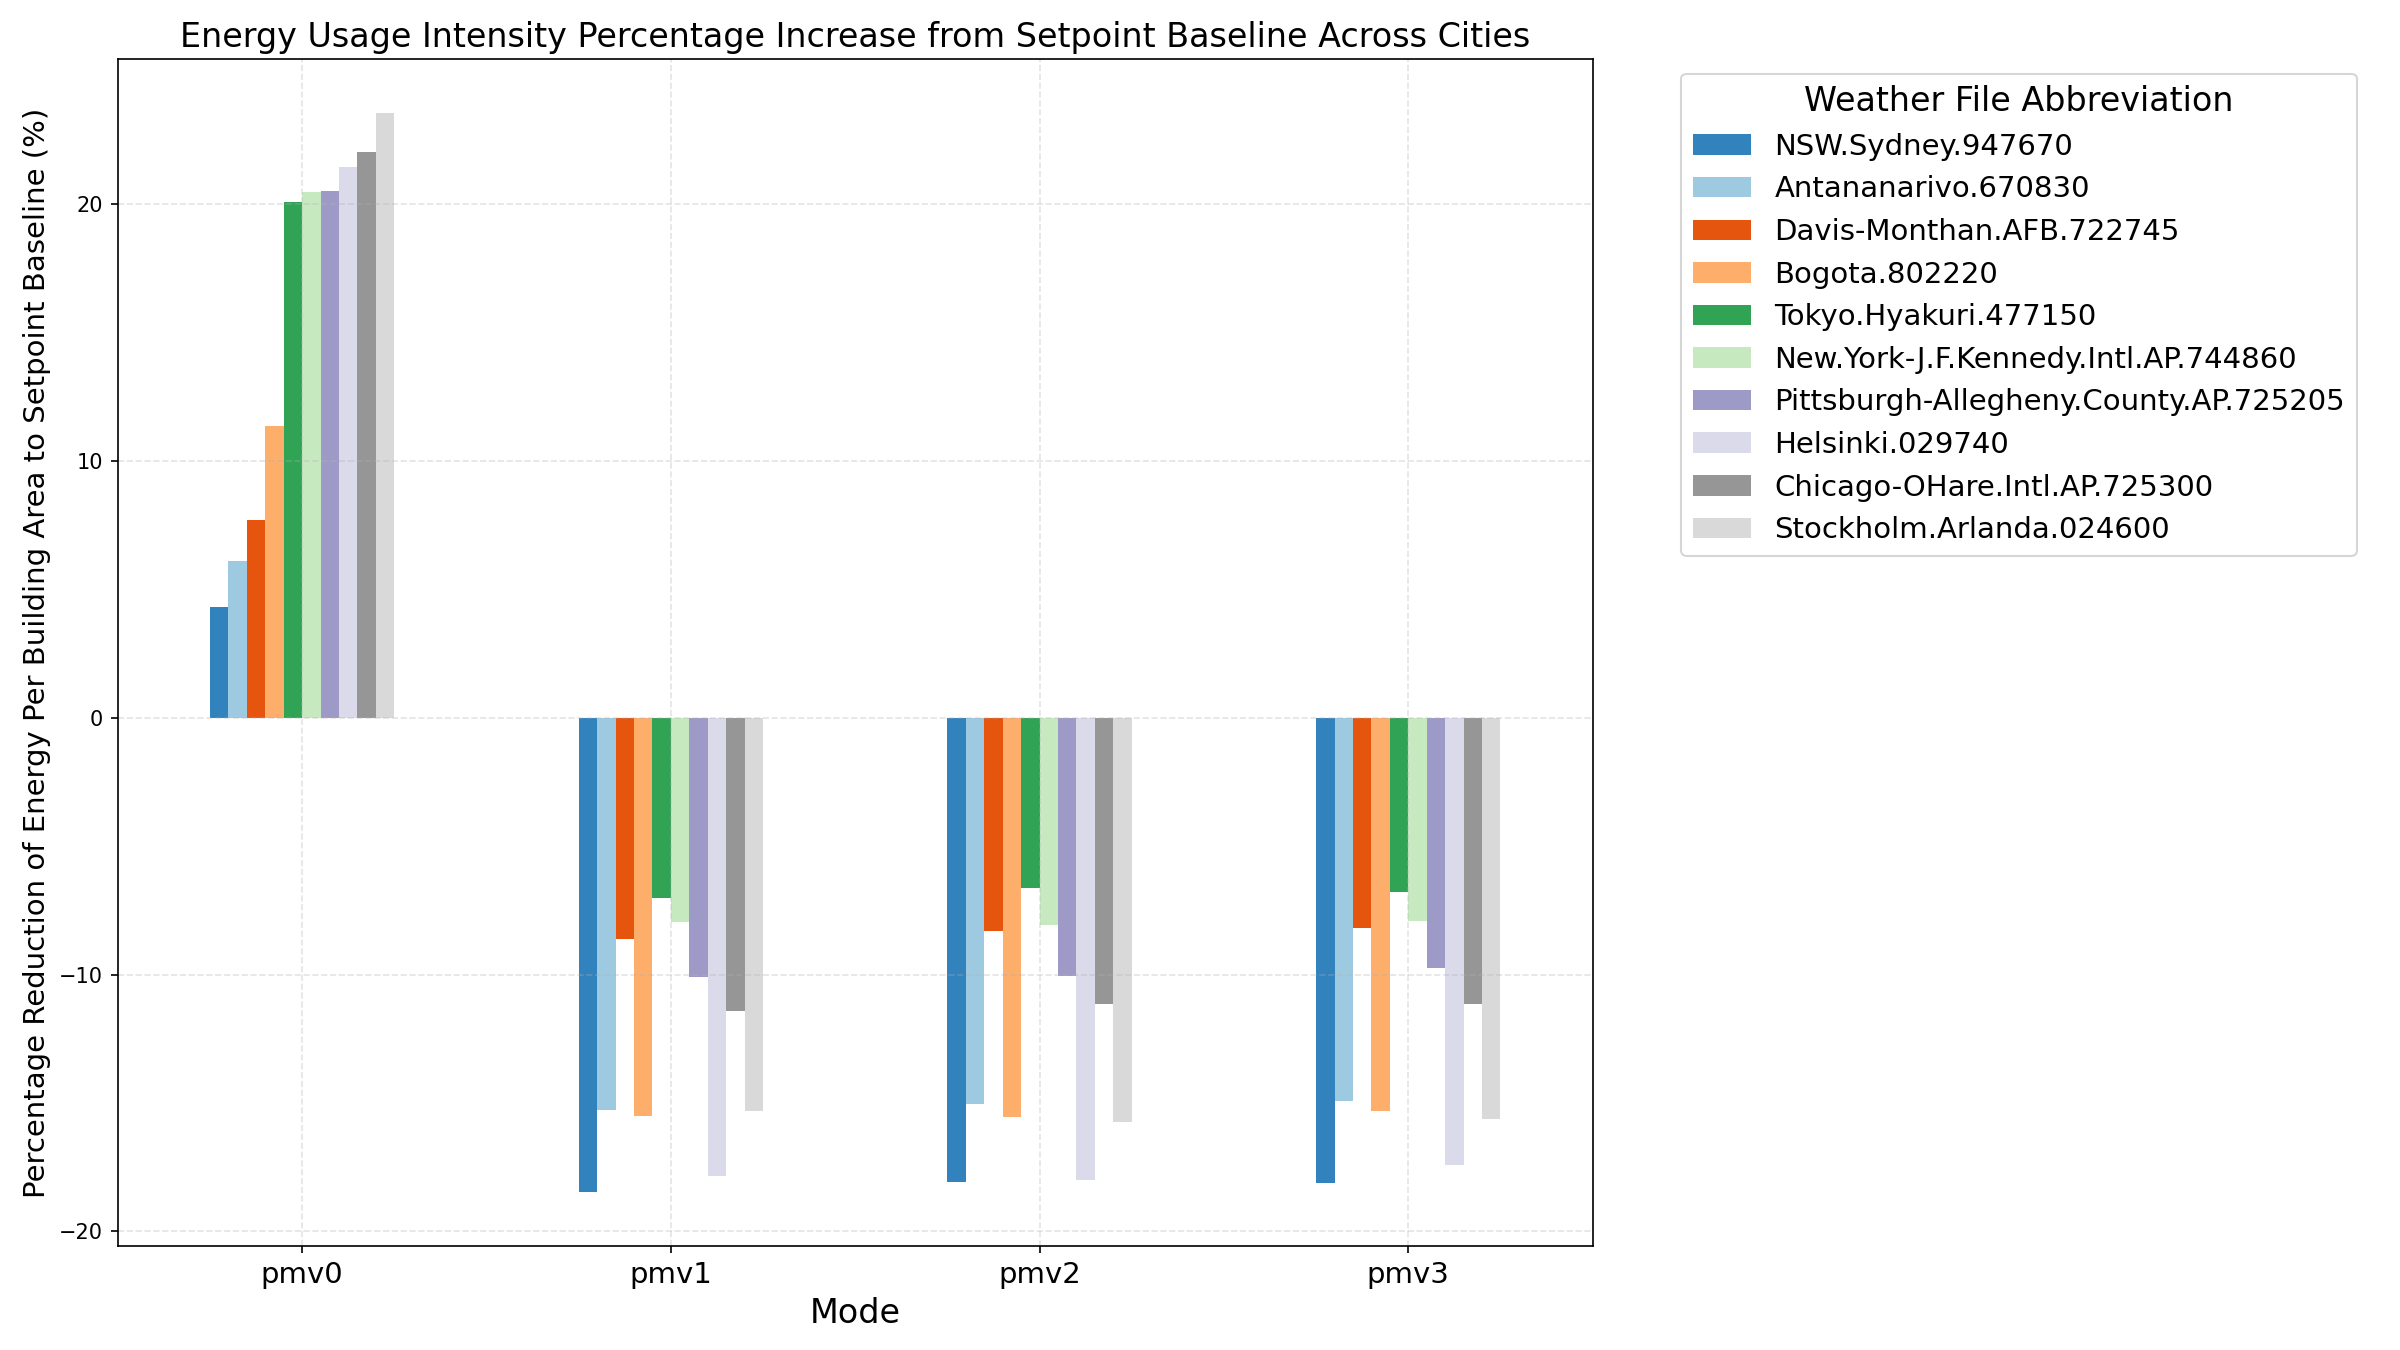
\includegraphics[width=0.85\linewidth]{figs/pmv_search_weather_perc.png}
    \caption{Energy Usage Intensity from EnergyPlus Simulations across multiple weather files (as specified with Figure~\ref{fig:workflow}}
    \label{fig:pmv-grid}
\end{figure}


\subsubsection{Observed Energy Savings with Grid-Search PMV Optimization}

In contrast to \texttt{pmv0}, the PMV-driven strategies employing grid-search optimization (\texttt{pmv1}, \texttt{pmv2}, \texttt{pmv3}), which incorporate different weightings for the energy/comfort trade-off and varied setpoint adjustment step sizes, demonstrated considerable success in reducing energy consumption relative to the bang-bang control.
\paragraph{Significant Savings (approx. 15\% to 18.5\% reduction):} Locations such as Helsinki ($ \approx -17.4\% \text{ to } -18.0\%$), Stockholm ($ \approx -15.3\% \text{ to } -15.8\%$), Sydney ($ \approx -18.1\% \text{ to } -18.5\%$), Bogota ($ \approx -15.3\% \text{ to } -15.6\%$), and Antananarivo ($ \approx -14.9\% \text{ to } -15.3\%$) fall into this category. These results are particularly prominent in climates with substantial heating seasons (Helsinki, Stockholm) but are also evident in the temperate oceanic climate of Sydney and the cooler subtropical highland climates. This suggests that intelligent PMV control can effectively capitalize on opportunities for energy reduction in varied conditions, possibly by optimizing system operation during significant heating/cooling periods or leveraging favorable ambient conditions in milder climates.

\paragraph{Consistent Savings (approx. 7\% to 11.5\% reduction):} Cities like Chicago ($ \approx -11.1\% \text{ to } -11.4\%$), Pittsburgh ($ \approx -9.8\% \text{ to } -10.1\%$), Davis-Monthan AFB ($ \approx -8.2\% \text{ to } -8.6\%$), New York ($ \approx -7.9\% \text{ to } -8.1\%$), and Tokyo ($ \approx -6.7\% \text{ to } -7.0\%$) showed this level of EUI reduction. These savings are observed in continental climates with distinct seasonal swings (Chicago, Pittsburgh, New York) as well as in a hot desert climate (Davis-Monthan) and a humid subtropical one (Tokyo). While the percentage is lower than the first group, the consistency across these demanding climates indicates the broad applicability and benefit of the grid-search PMV approach. Even in cooling-dominated or highly humid environments, these strategies identify pathways to improved efficiency over basic control. 

\begin{figure}[h!]
    \centering
    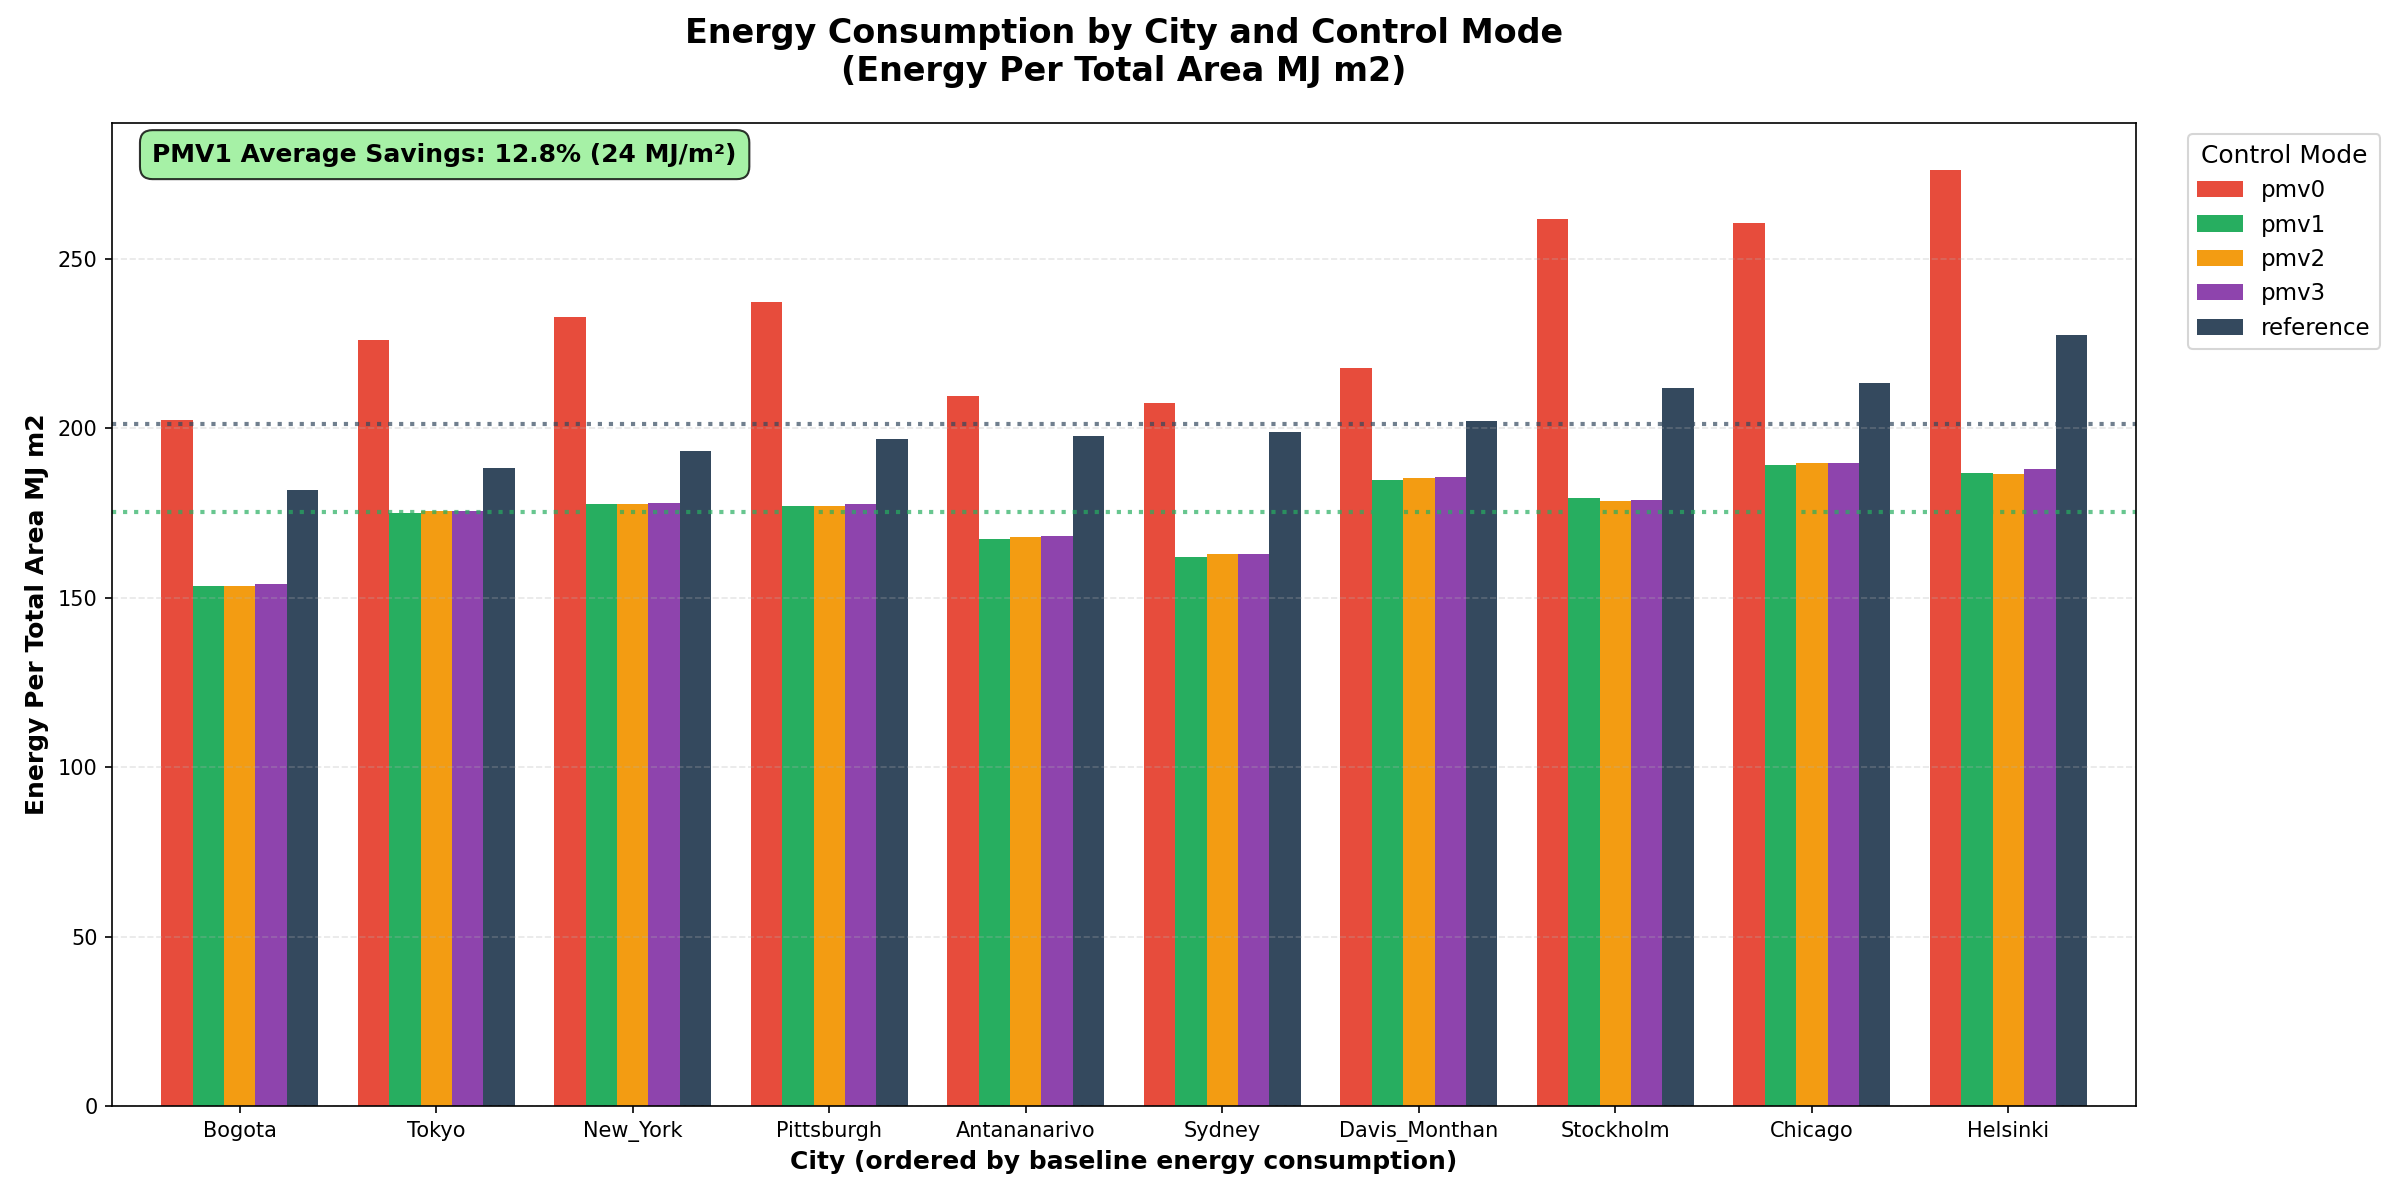
\includegraphics[width=0.95\linewidth]{figs/Energy_Per_Total_Area_MJ_m2_pmv.png}
    \caption{Energy per total area savings across all climates between reference state and all PMV-based control mode variations.}
    \label{fig:MJm2pmv}
\end{figure}

This can be better seen in Figure~\ref{fig:MJm2pmv}, where grid-search approach (\texttt{pmv1}, \texttt{pmv2}, \texttt{pmv3}) is broadly helpful and effective in achieving energy savings. These strategies consistently outperformed both the reference bang-bang control and the simplistic \texttt{pmv0} strategy. Optimized PMV-based control achieved consistent energy savings (averaging at around 12.75\% for PMV1), notably matching ML-based controls. This highlights the unexpected yet robust efficiency achievable by classical comfort models when systematically optimized.

The results clearly highlight that the grid-search approach (pmv1, pmv2, pmv3) is broadly helpful and effective in achieving energy savings. These strategies consistently outperformed both the reference bang-bang control and the simplistic pmv0 strategy. Notably, the three grid-search variants yielded remarkably similar energy savings within each city—typically varying by only one or two percentage points—suggesting that the underlying framework of PMV-based grid search with energy/comfort trade-offs is inherently robust. This convergence in performance indicates there is no single "one-solution-fits-all" strategy among pmv1, pmv2, and pmv3 that consistently yields superior energy results across all diverse climates. While all are effective, the specific parameters (weights, step sizes) explored in these variants might lead to different comfort experiences for occupants, which is not captured in this EUI data but would be a critical consideration for practical implementation. The choice among these similar-performing strategies might ultimately hinge on their differential impact on occupant comfort or other operational considerations beyond pure energy efficiency.

Optimized PMV controls consistently achieved significant (15–18.5\%) or moderate (7–11.5\%) energy savings across diverse climates, demonstrating robust performance independent of geographic and climatic variations. This highlights that grid-search optimization of classical comfort models effectively balances comfort and energy efficiency, rivaling sophisticated ML models.

\subsubsection{Observed Energy Savings with Grid‐Search PMV Optimization}
\label{sec:pmv_energy}

Figure~\ref{fig:stockholm-tokyo} illustrates how the \texttt{pmv1} grid‐search control exploits climatic differences to widen the neutral comfort band. In Stockholm’s cold‐continental summer, lower humidity allows indoor temperatures to reach 27–28\,$^\circ$C (a 5–7\,$^\circ$C expansion from the baseline) without violating PMV neutrality, effectively utilizing `free cooling' from economizer mode operation from June through September. Tokyo's humid-subtropical summer climate restricts this expansion to only 2–3\,$^\circ$C (25–26\,$^\circ$C) due to higher humidity levels that affect thermal comfort. The PMV1 algorithm inherently recognizes these psychrometric constraints and maintains setpoint extremes until indoor conditions approach the boundaries of the expanded comfort range (see Figure~\ref{fig:zoomed-tkst}), resulting in extended economizer mode operation and substantial annual energy reductions without compromising occupant comfort.

\begin{figure}[h!]
    \centering
    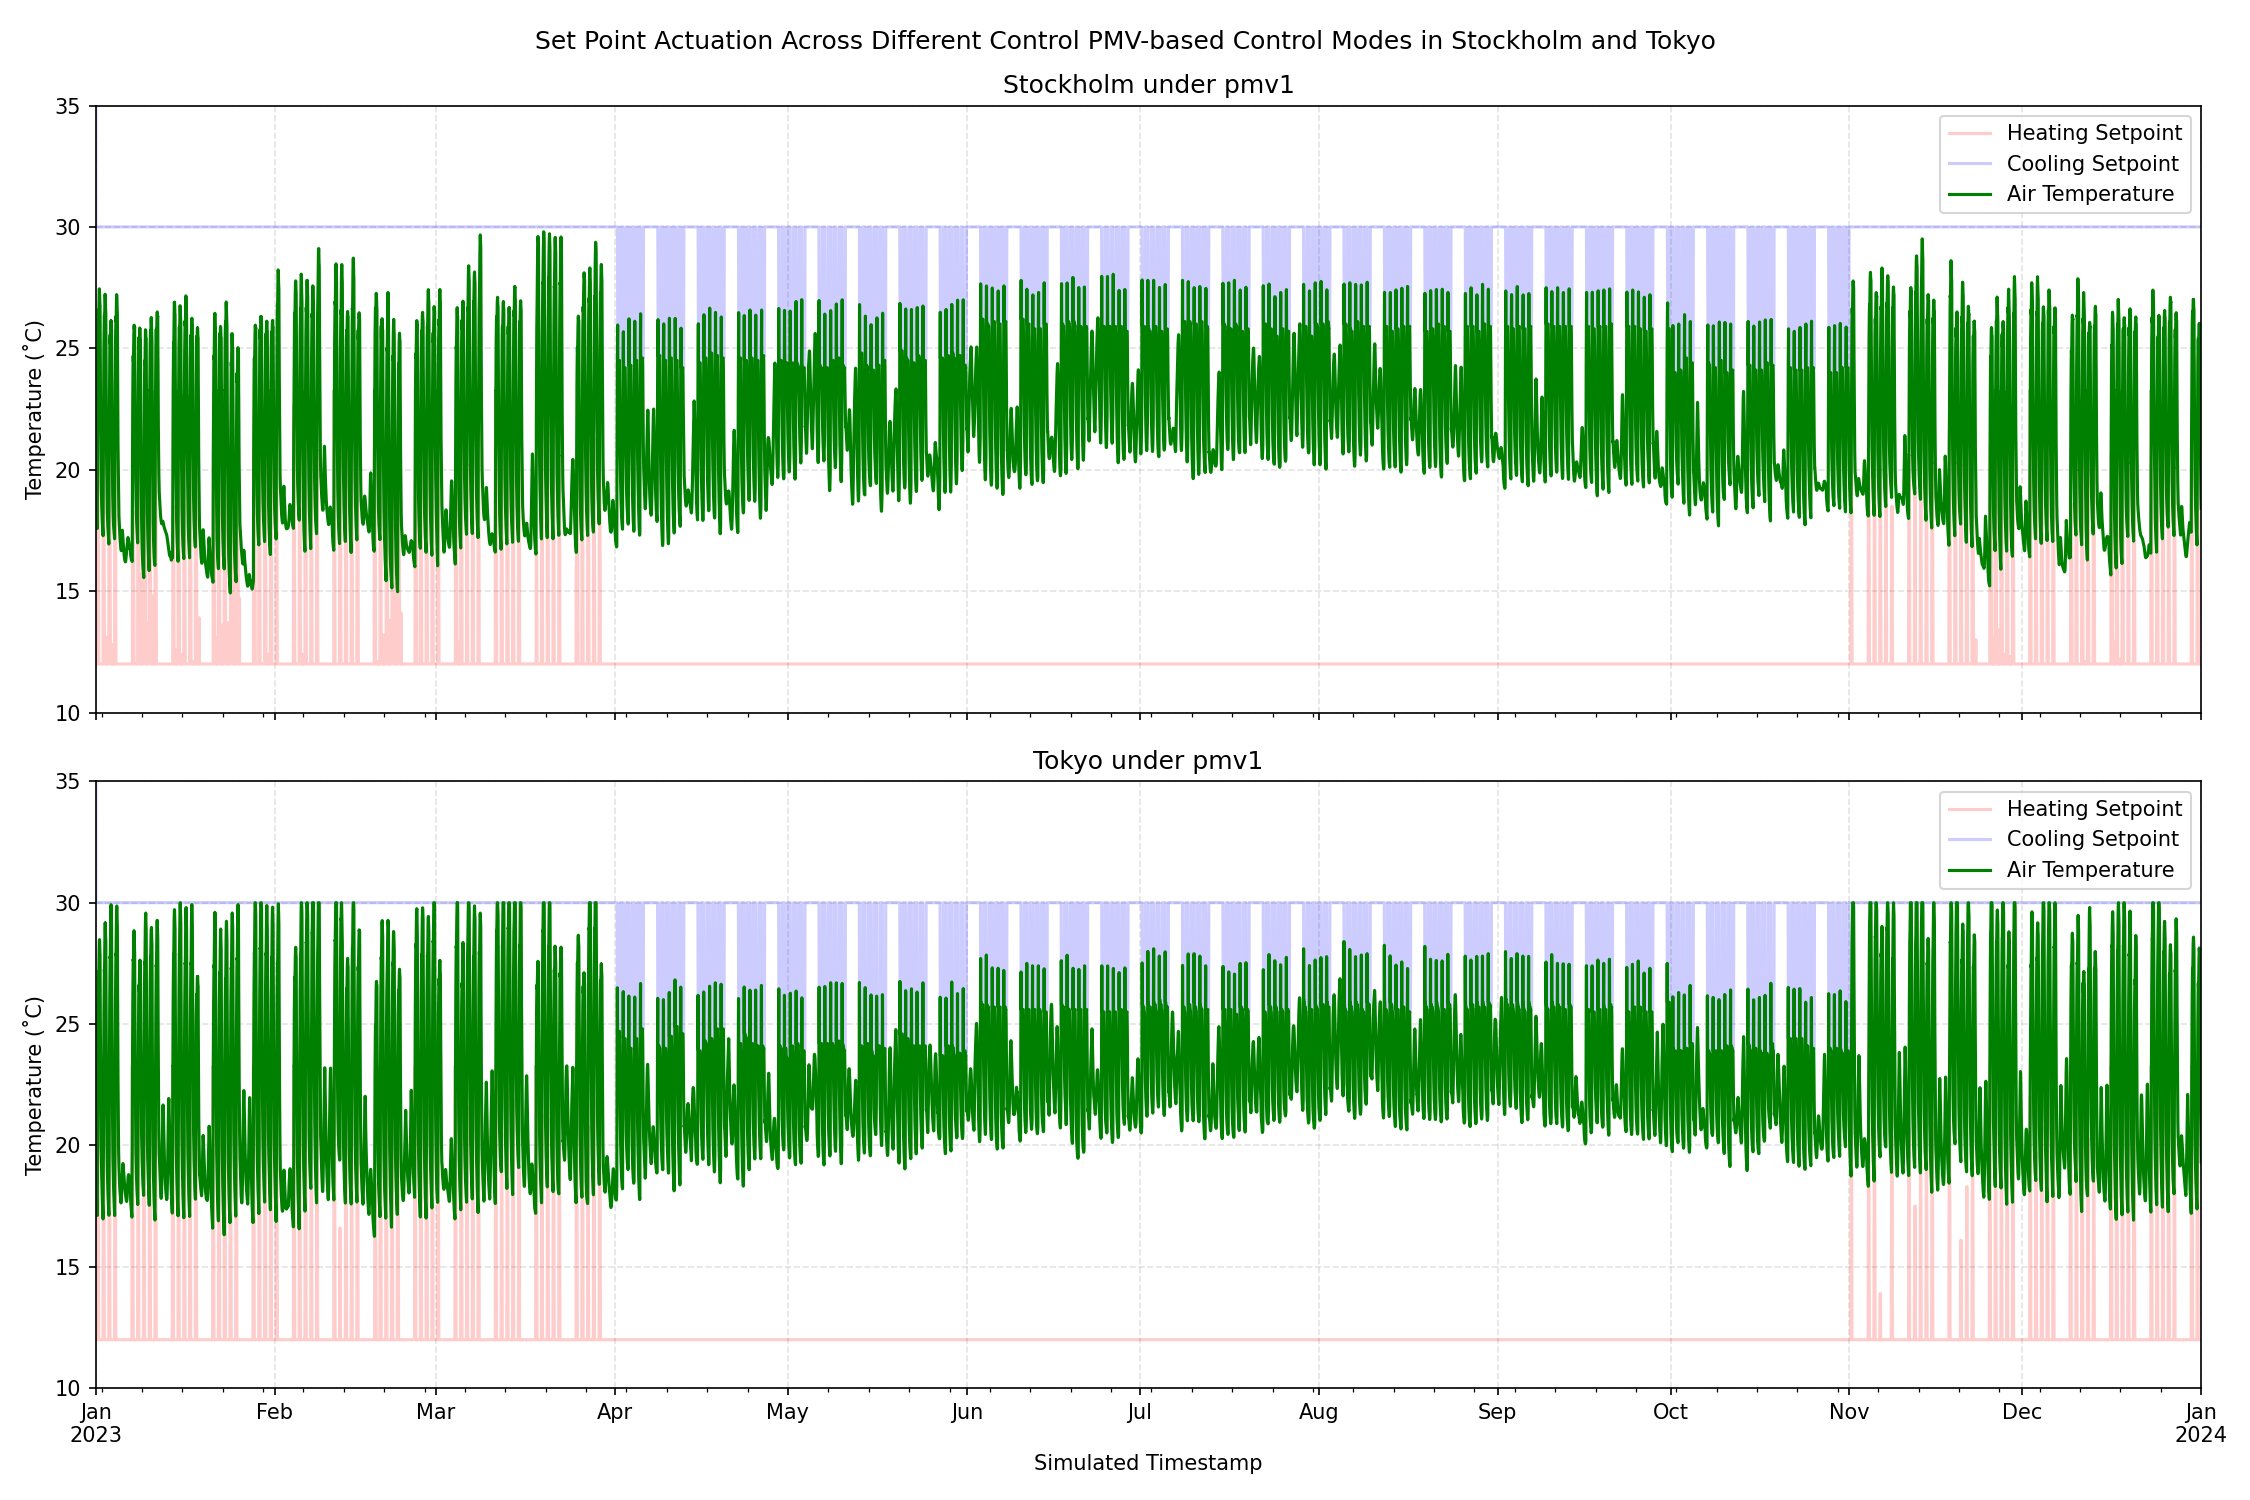
\includegraphics[width=0.95\linewidth]{figs/Stockholm_Tokyo.png}
    \caption{PMV1 control adaptation in contrasting climates: (a) Stockholm’s lower summer humidity permits indoor setpoints of 27–28\,$^\circ$C while maintaining PMV neutrality; (b) Tokyo’s higher humidity constrains summer setpoints to 25–26\,$^\circ$C.}
    \label{fig:stockholm-tokyo}
\end{figure}

\begin{figure}[h!]
    \centering
    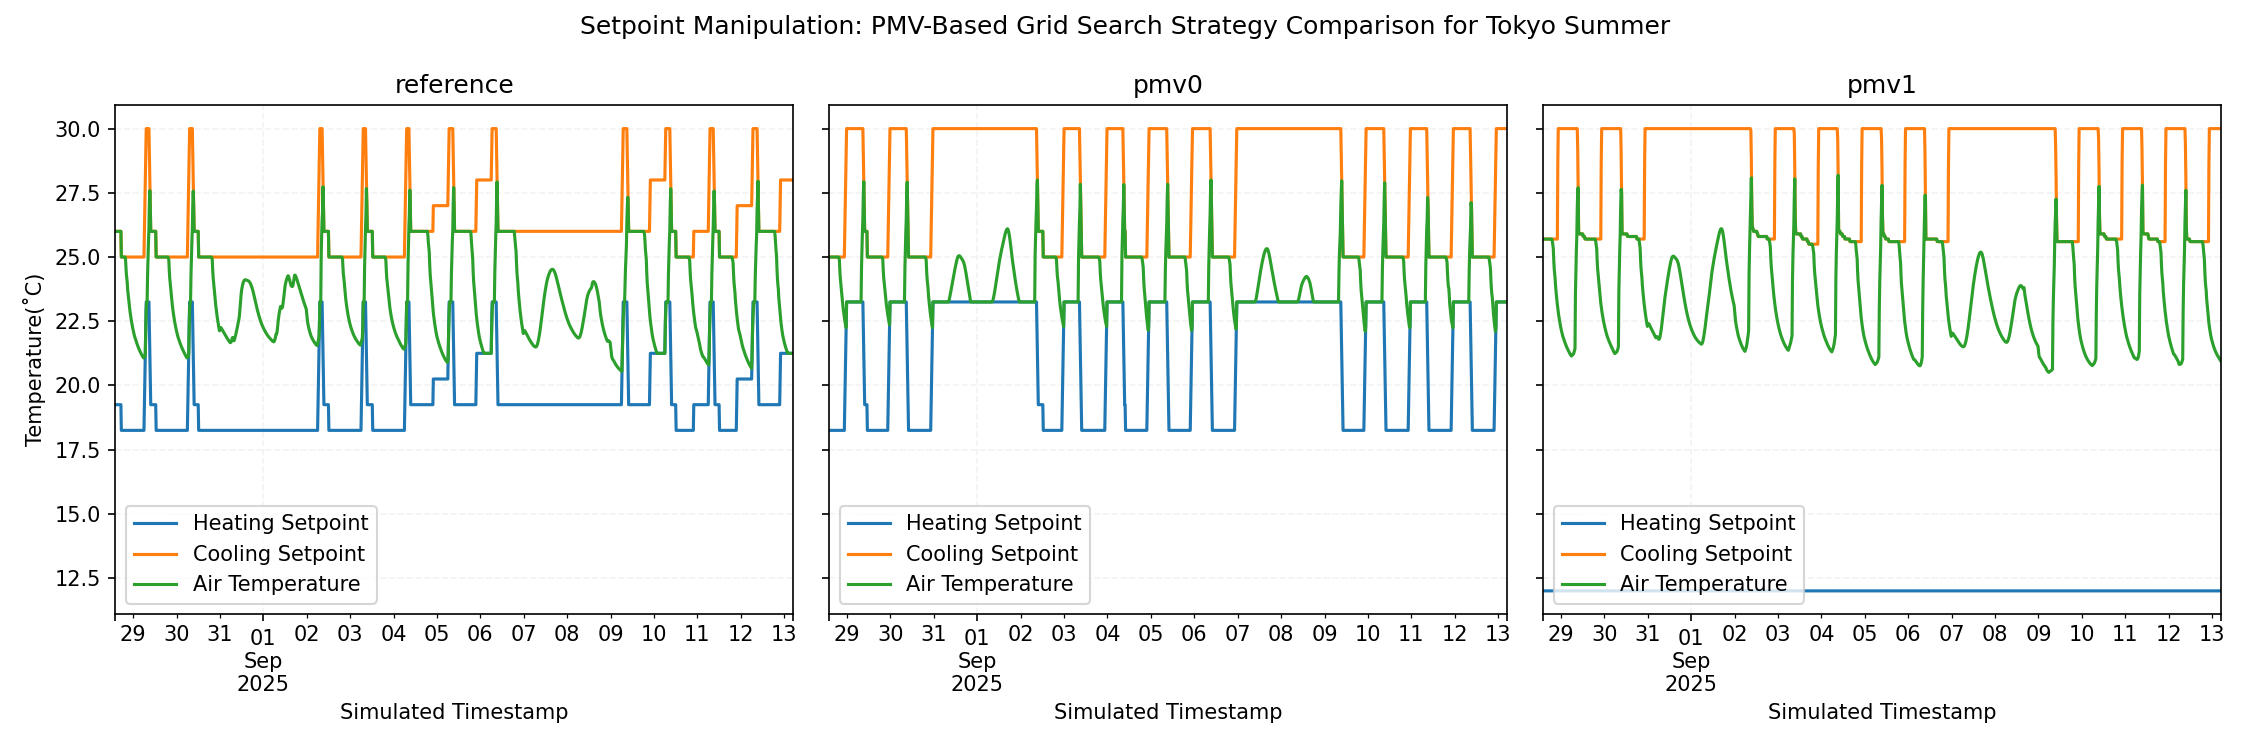
\includegraphics[width=0.75\linewidth]{figs/realcontrol_tk.png}
    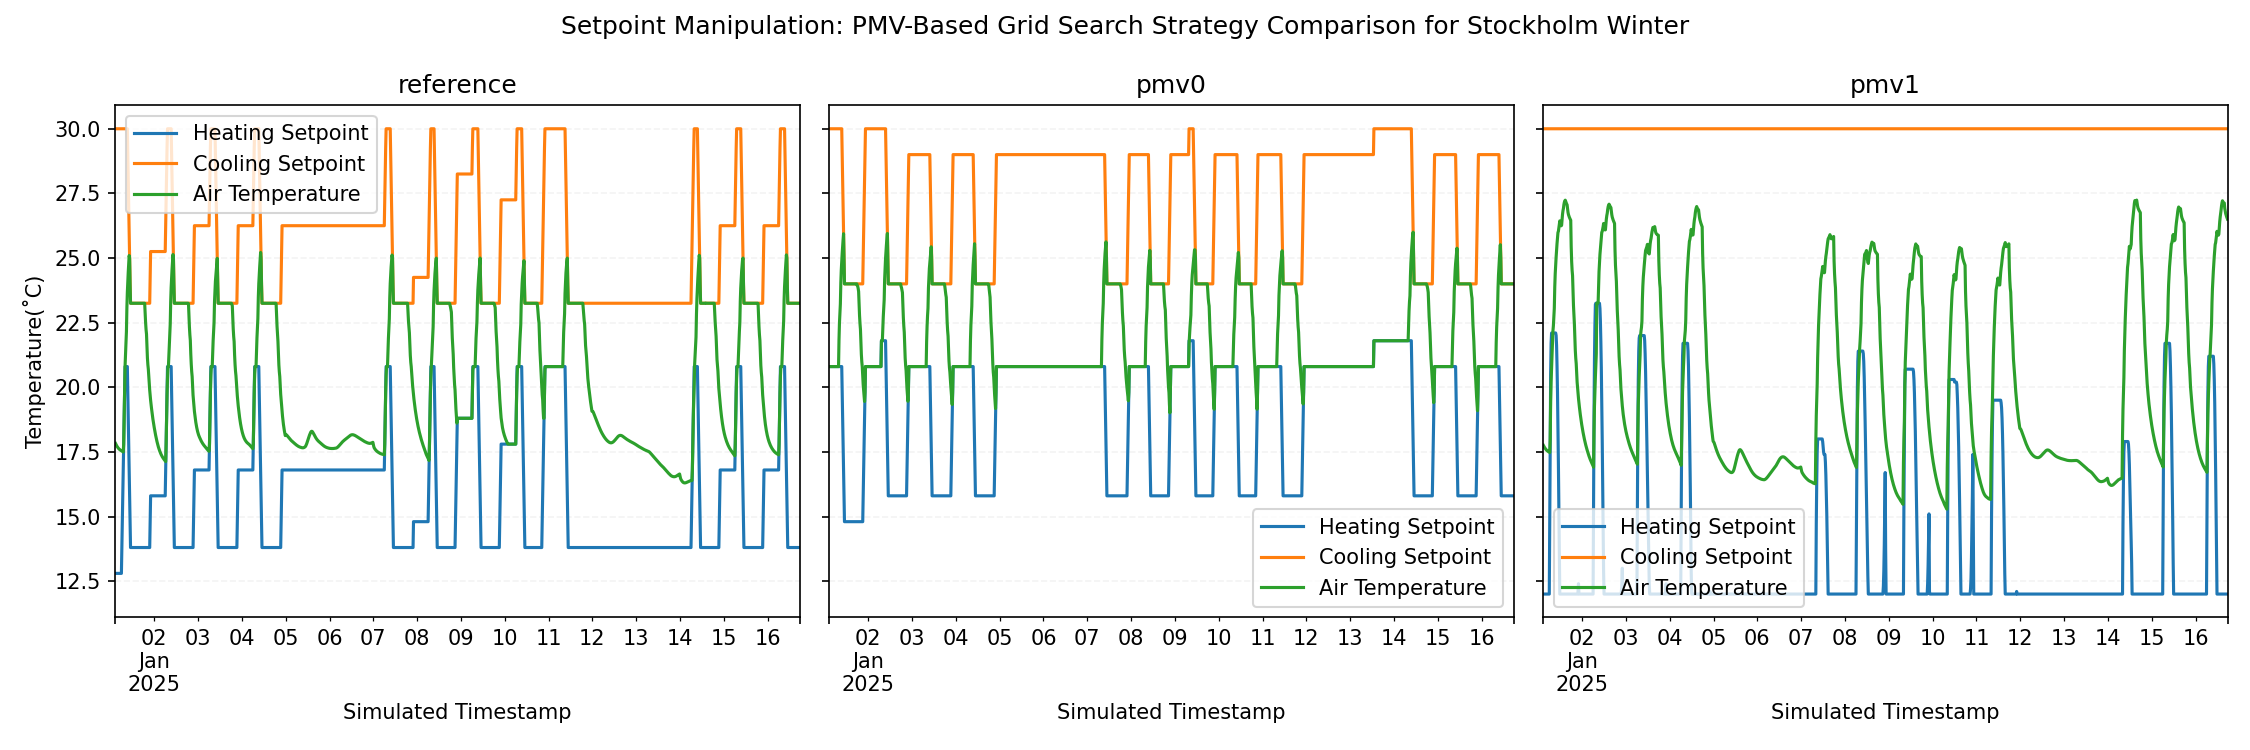
\includegraphics[width=0.75\linewidth]{figs/realcontrol_st.png}
    \caption{Detailed setpoint behavior under PMV1: (top) Tokyo summer holds cooling at the grid‐searched maximum until indoor temperature drifts outside the widened band; (bottom) Stockholm winter holds heating at the minimum as passive gains maintain comfort.}
    \label{fig:zoomed-tkst}
\end{figure}

\subsection{Control Strategy Comparison}
\label{sec:all_control_strategies}
As outlined in the methodology, we compared the seven different control scenarios across four different weather files within our selected IDF file, where we analyze their corresponding energy usage, thermal comfort status, and overall runtime. Figure~\ref{fig:runtime} presents the runtime comparison between the 7 control scenarios. As anticipated, the reference case is consistently the fastest, typically completing annual simulations in 15-20 seconds with no external components to communicate. PMV shows comparable performance at similar runtimes since it's also an analytical model using deterministic calculations. The machine learning models show significantly longer runtimes. LightGBM takes approximately 150-200 seconds per simulation—roughly 10 times slower than reference/PMV—due to model loading and prediction for anticipated occupant arrays. PINN-VAE demonstrates even longer runtimes at 600-900 seconds, as deep learning models require more computational overhead despite vectorized processing.

\begin{figure}[h!]
    \centering
    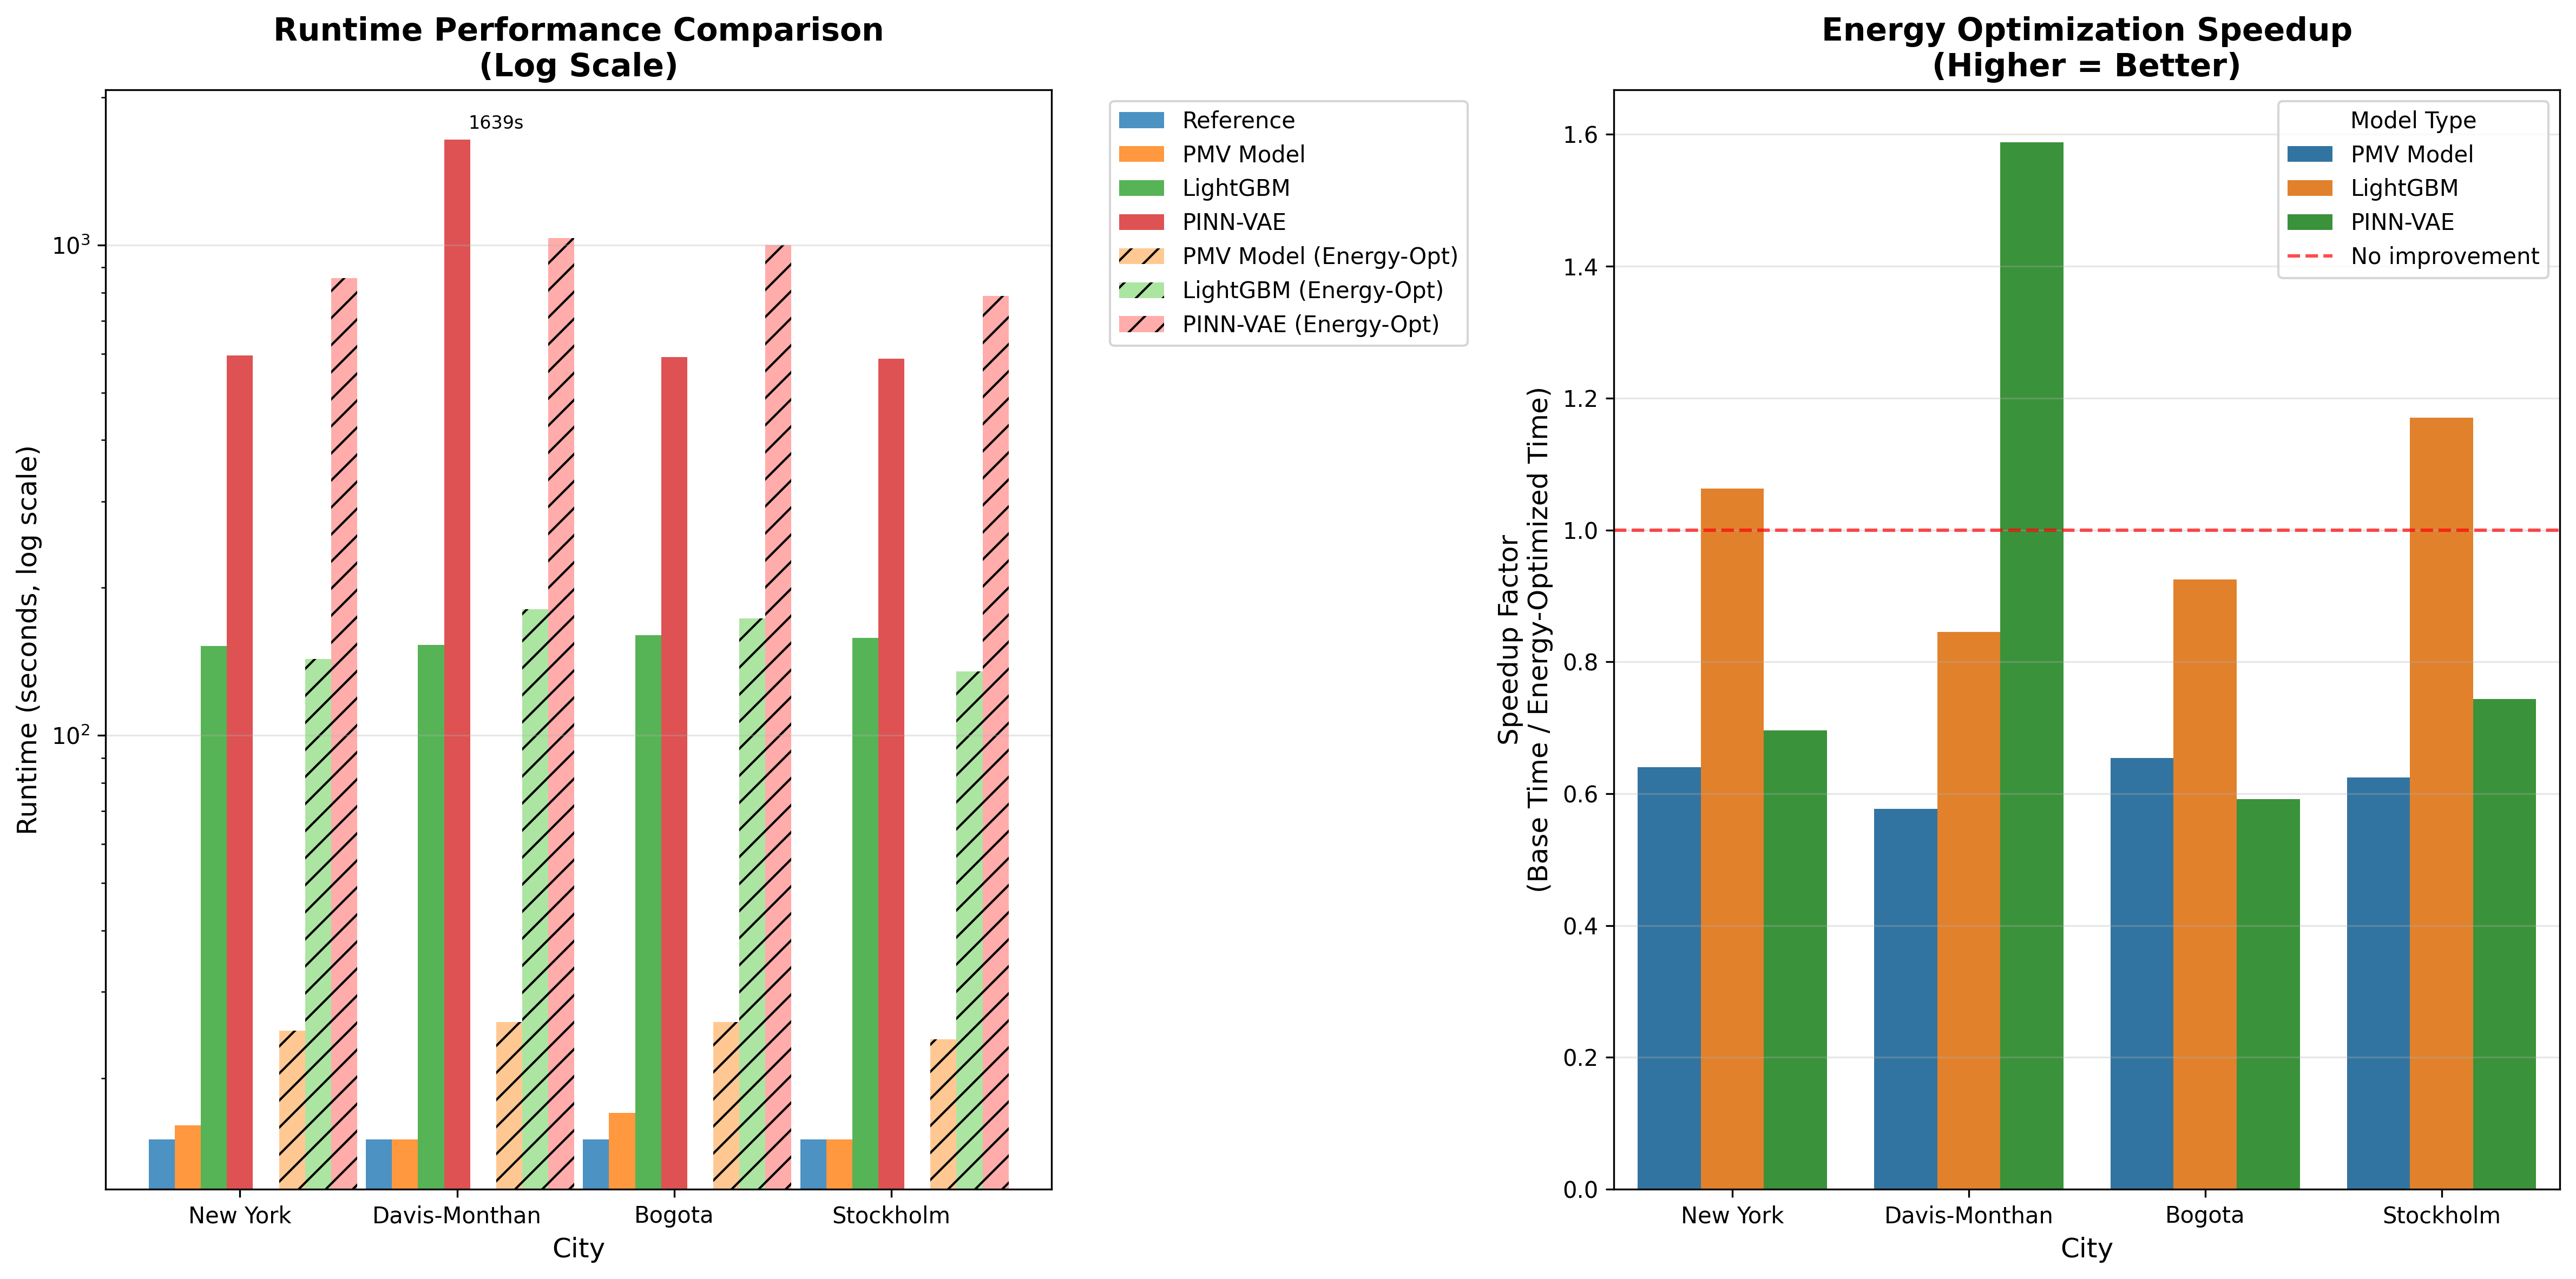
\includegraphics[width=0.75\linewidth]{figs/runtime.png}
    \caption{Runtime comparison between different thermal sensation prediction base models and computational time increase from implicit energy-saving $\Delta T$ grid search.}
    \label{fig:runtime}
\end{figure}

In contrast, the grid search optimization (`-o' variants) reveals interesting patterns: for PMV and LightGBM, the grid search approximately doubles runtime compared to their base versions, reflecting the computational cost of evaluating multiple temperature offset scenarios. However, PINN-VAE shows minimal runtime increase with optimization (comparing `pv' to `pv-o'), suggesting that model inference time dominates over the additional grid search computations. These runtime differences have important implications for real-time control applications, where the sub-200 second performance of optimized PMV and LightGBM remains practical, while PINN-VAE's 10-15 minute runtimes may limit its deployment to offline optimization scenarios.

\subsubsection{Energy Usage and Thermal Comfort Statistics}
\label{sec:energy_comfort_analysis}
This section analyzes the quantitative energy and comfort outcomes of each control strategy, examining total consumption, component-level breakdowns, and thermal comfort distributions.
We first examine the energy and comfort performance of each control strategy. Figure~\ref{fig:energy_ranking} presents the annual energy consumption ranking (1 = most efficient) for each control mode in Bogota, Davis‐Monthan, New York, and Stockholm. Across all four climates, the optimized grid‐search variants (\texttt{pmv-o}, \texttt{lightgbm-o}, \texttt{pv-o}) consistently occupy the top three positions, demonstrating robust, climate‐independent performance. In contrast, the “pure” modes (\texttt{pmv}, \texttt{lightgbm}, \texttt{pv}) occupy the lower ranks (5–7), despite sometimes achieving localized cooling or fan energy reductions. This discrepancy arises because unoptimized controllers frequently request setpoints beyond the 12 $^\circ$C–30 $^\circ$C limits, leading to actuator clipping and spurious energy savings in one end use that are more than offset by large energy penalties in another. The baseline \texttt{reference} (`bang–bang') control invariably sits in the middle (rank 4), underscoring that naïve comfort‐based inversions can underperform a simple hysteresis thermostat when actuator saturation is not considered.

\begin{figure}[h!]
    \centering
    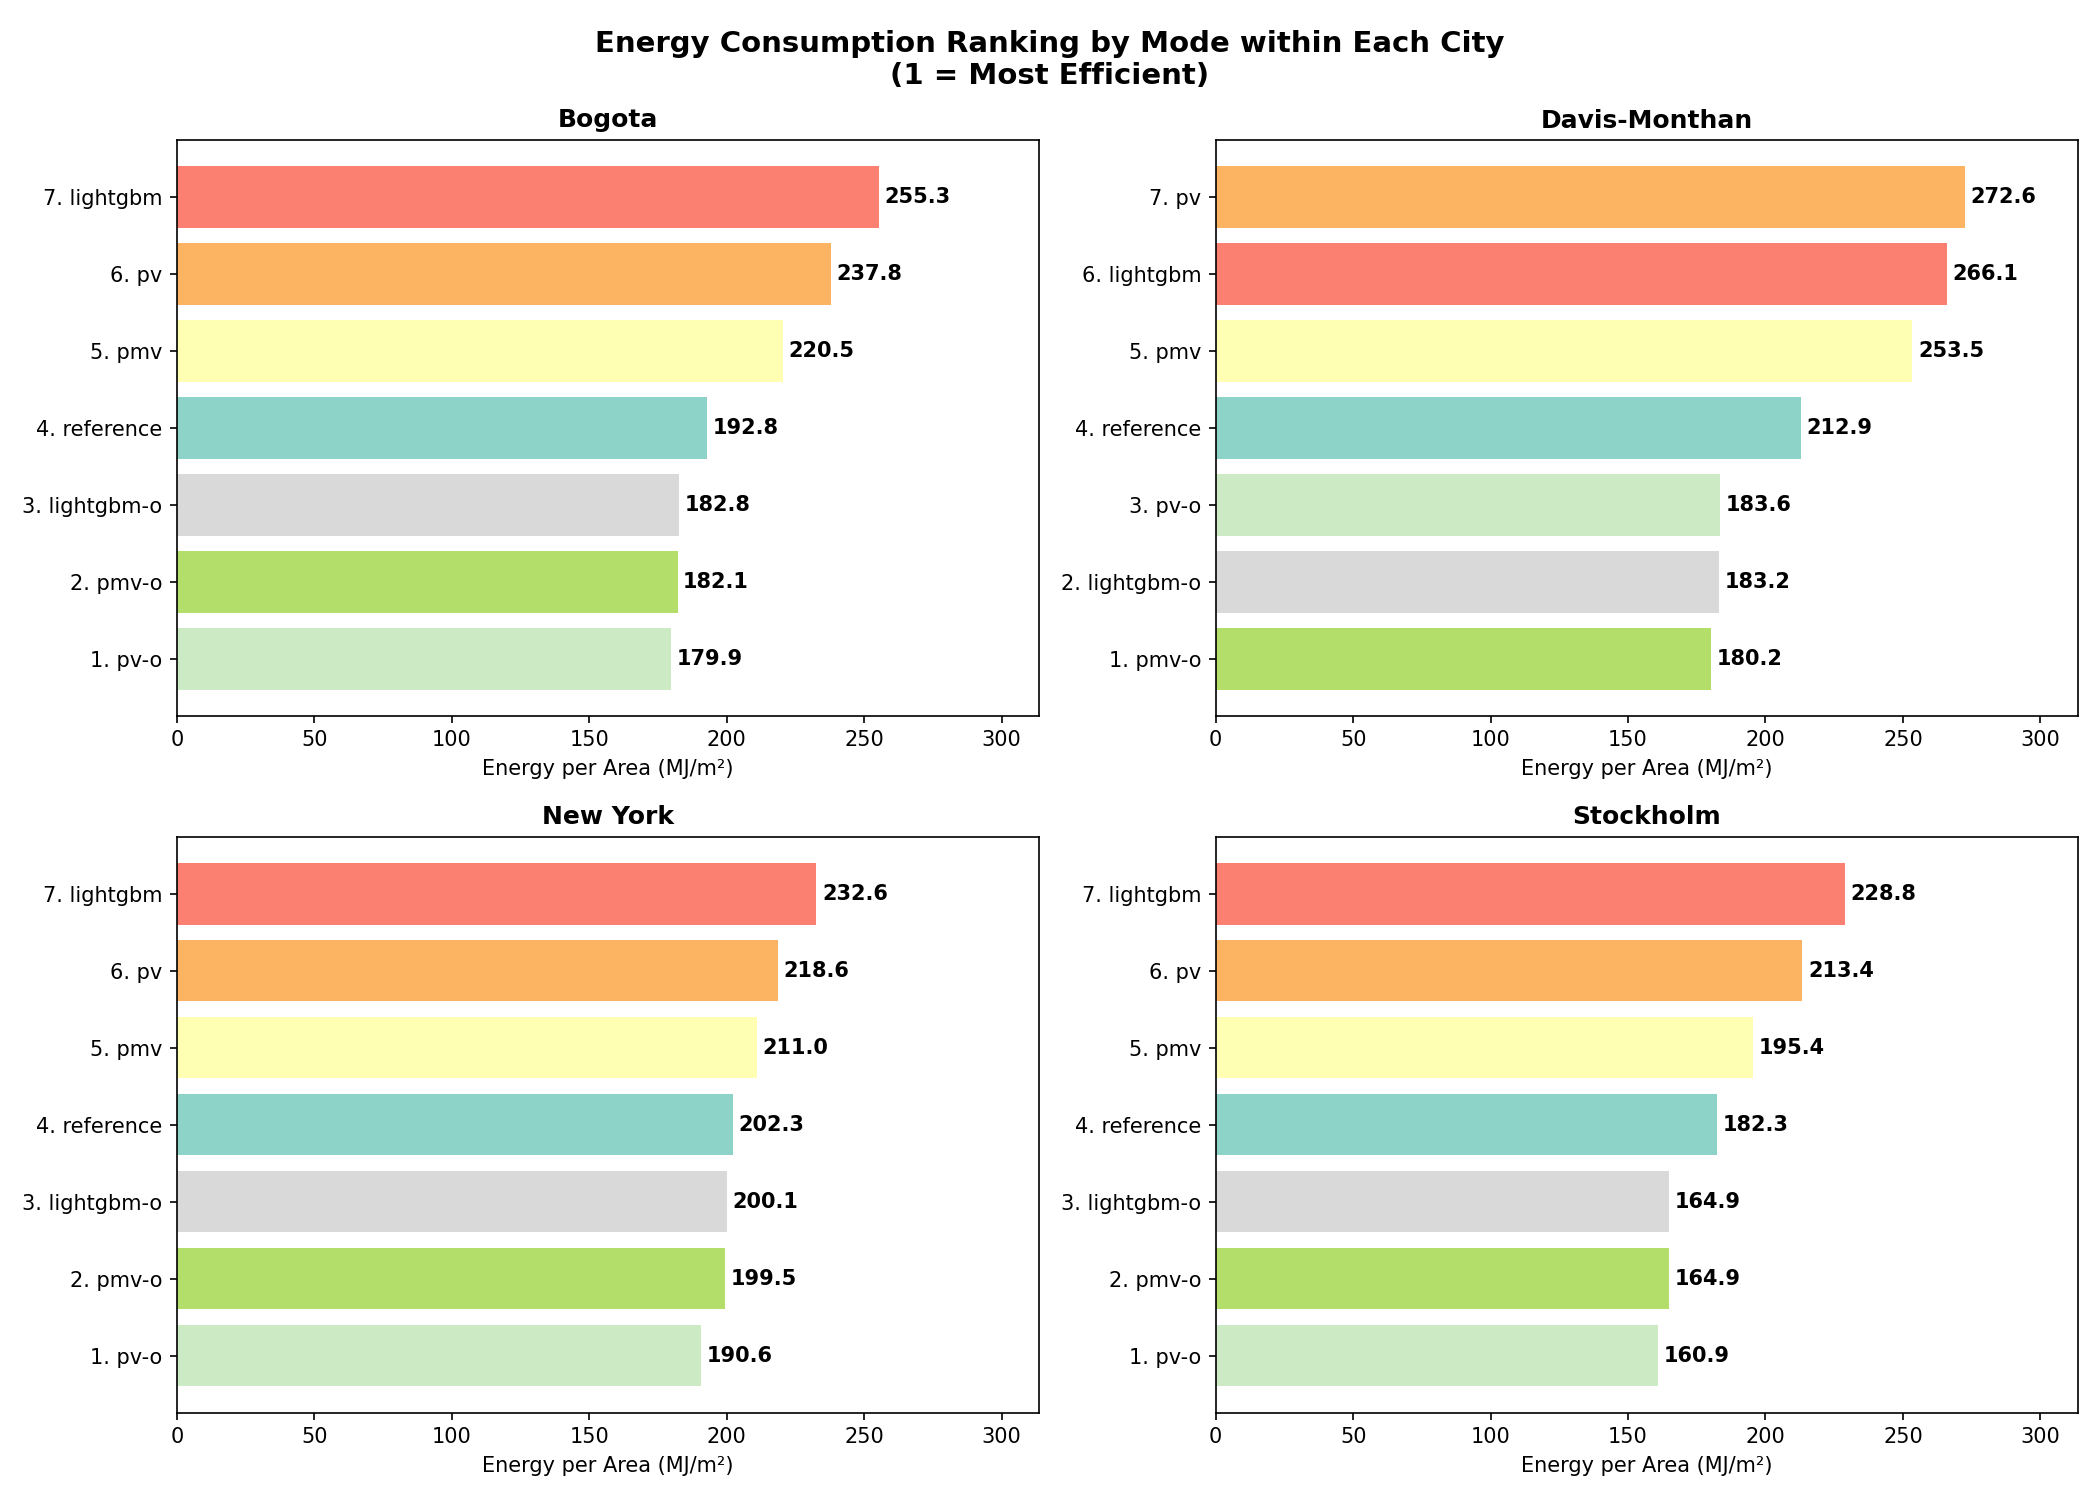
\includegraphics[width=\linewidth]{figs/energy_consumption_ranking_by_mode_within_each_city.png}
    \caption{Energy consumption ranking (1 = most efficient) for each control mode in four cities. Grid‐search variants (\texttt{pmv-o}, \texttt{lightgbm-o}, \texttt{pv-o}) occupy the top three ranks, while unoptimized “pure” modes (\texttt{pmv}, \texttt{pv}, \texttt{lightgbm}) lie at the bottom.}
    \label{fig:energy_ranking}
\end{figure}

Figure~\ref{fig:thermal_comfort} compares thermal comfort (Predicted Mean Vote, PMV) and indoor temperature distributions across all seven modes in the same four cities. The grid‐search variants maintain median PMV values tightly within the neutral band (–0.5 to +0.5) and exhibit markedly smaller interquartile ranges than the pure modes. For example, \texttt{pv-o} and \texttt{pmv-o} rarely exceed $\pm$0.5, indicating consistent comfort despite varying external conditions. By contrast, \texttt{lightgbm} and \texttt{pv} without optimization show bimodal PMV distributions, with frequent excursions above +1.0 or below –1.0, reflecting repeated setpoint clipping at 12$^\circ$C or 30$^\circ$C. These clipping‐induced comfort violations correspond to the oscillatory indoor temperature patterns visible in the lower panel: the pure ML/PV modes force indoor air to swing between the extremes of 12$^\circ$C and 30$^\circ$C, whereas grid‐search controllers keep most of their temperatures in the 22–26$^\circ$C range. This stabilization of indoor conditions not only preserves occupant comfort but also eliminates the energy wasted on cycling between extremes.

\begin{figure}[h!]
    \centering
    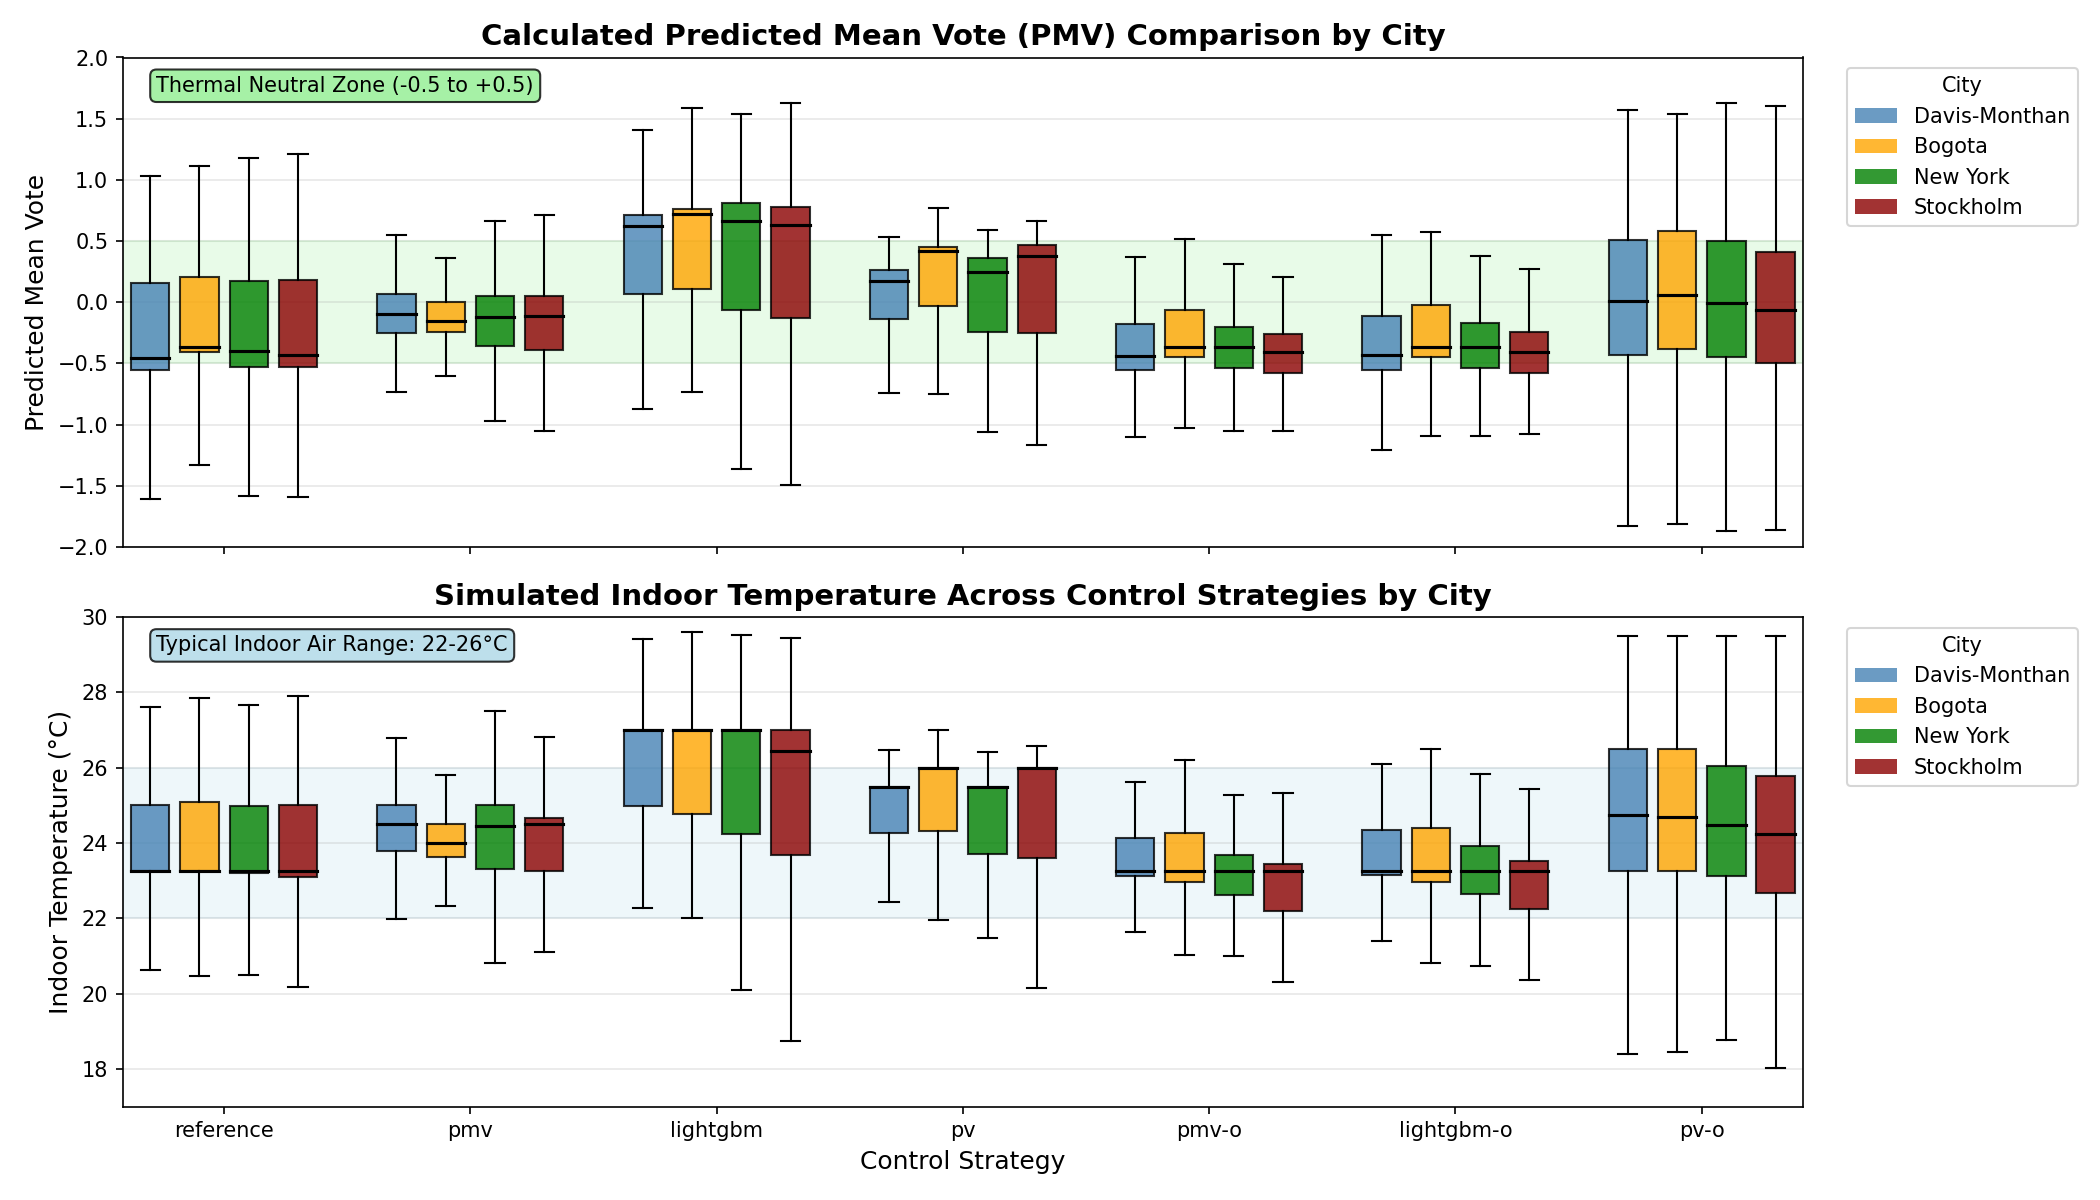
\includegraphics[width=\linewidth]{figs/thermal_comfort_comparison_improved.png}
    \caption{Top: PMV distributions by control mode and city (green shading = comfort zone, $\pm$0.5). Bottom: Indoor temperature distributions (blue shading = typical comfort range, 22–26$^\circ$C). Grid‐search variants exhibit tighter comfort control and avoid clipping‐induced extremes.}
    \label{fig:thermal_comfort}
\end{figure}

Figure~\ref{fig:component_savings} breaks down energy savings (relative to \texttt{reference}) into heating, cooling, and fan components for each city. The grid‐search PMV variant (\texttt{pmv-o}) achieves the largest heating reductions—up to +91\% in Bogota and +79\% in Davis—by tolerating expanded neutral temperature bands in summer and leveraging passive gains in winter. Although \texttt{pmv-o} incurs small negative cooling savings in colder climates (e.g., –16\% in Stockholm), the net effect is still a substantial reduction in overall HVAC energy. Similarly, \texttt{lightgbm-o} and \texttt{pv-o} realize significant heating savings (+58\% to +75\%) with modest cooling trade‐offs. In contrast, the unoptimized \texttt{lightgbm} and \texttt{pv} modes display large negative heating “savings”—for instance, –889\% in Davis and –295\% in New York—because they remain pinned at 12$^\circ$C during extremes and then must repeatedly reheat, creating enormous energy penalties. Their apparent cooling or fan energy gains are insufficient to offset these heating losses, confirming that actuator clipping can produce misleading component‐level metrics.

\begin{figure}[h!]
    \centering
    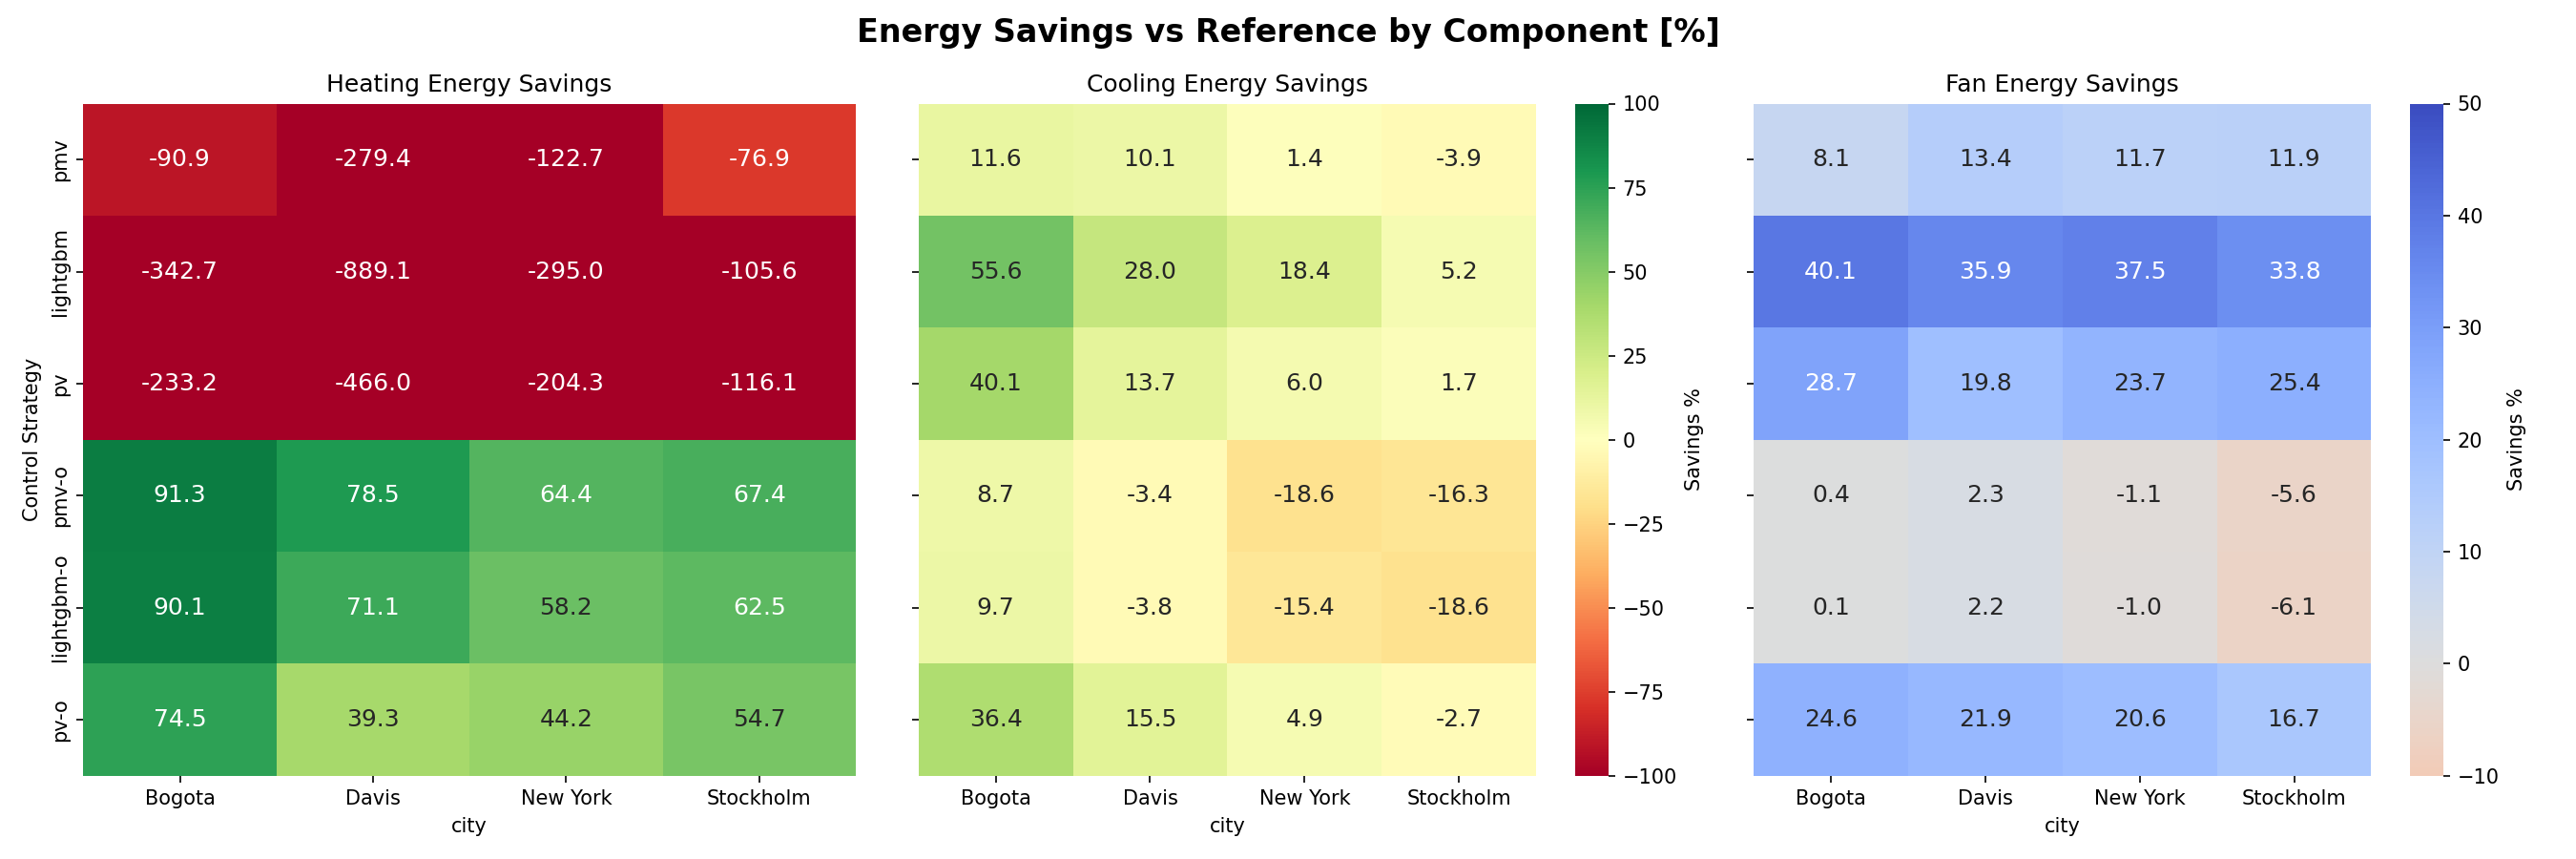
\includegraphics[width=\linewidth]{figs/saving_end_pct.png}
    \caption{Component‐level energy savings (\%) relative to \texttt{reference}, by city and control mode. Positive values indicate reduced consumption. Grid‐search variants (\texttt{pmv-o}, \texttt{lightgbm-o}, \texttt{pv-o}) achieve large heating savings with minor cooling/fan trade‐offs, while pure modes incur large heating penalties due to clipping.}
    \label{fig:component_savings}
\end{figure}

When aggregated into total HVAC energy savings (Figure~\ref{fig:hvac_savings}), grid‐search variants consistently deliver substantial net reductions—from 90\% in Bogota to 62\% in Stockholm—highlighting the method’s ability to achieve “win–win” outcomes: maintaining neutral PMV and stable indoor temperatures while dramatically lowering energy use. In contrast, pure \texttt{lightgbm} and \texttt{pv} modes produce negative net savings across all climates (e.g., –466\% in Davis, –204\% in New York), reflecting their pathological reliance on setpoints clipped to extremes. The \texttt{reference} controller (0\% savings by definition) outperforms unoptimized pure modes in some climates, underscoring that a simplistic hysteresis thermostat can surpass naïve comfort‐driven logic when actuator saturation is unresolved.

\begin{figure}[h!]
    \centering
    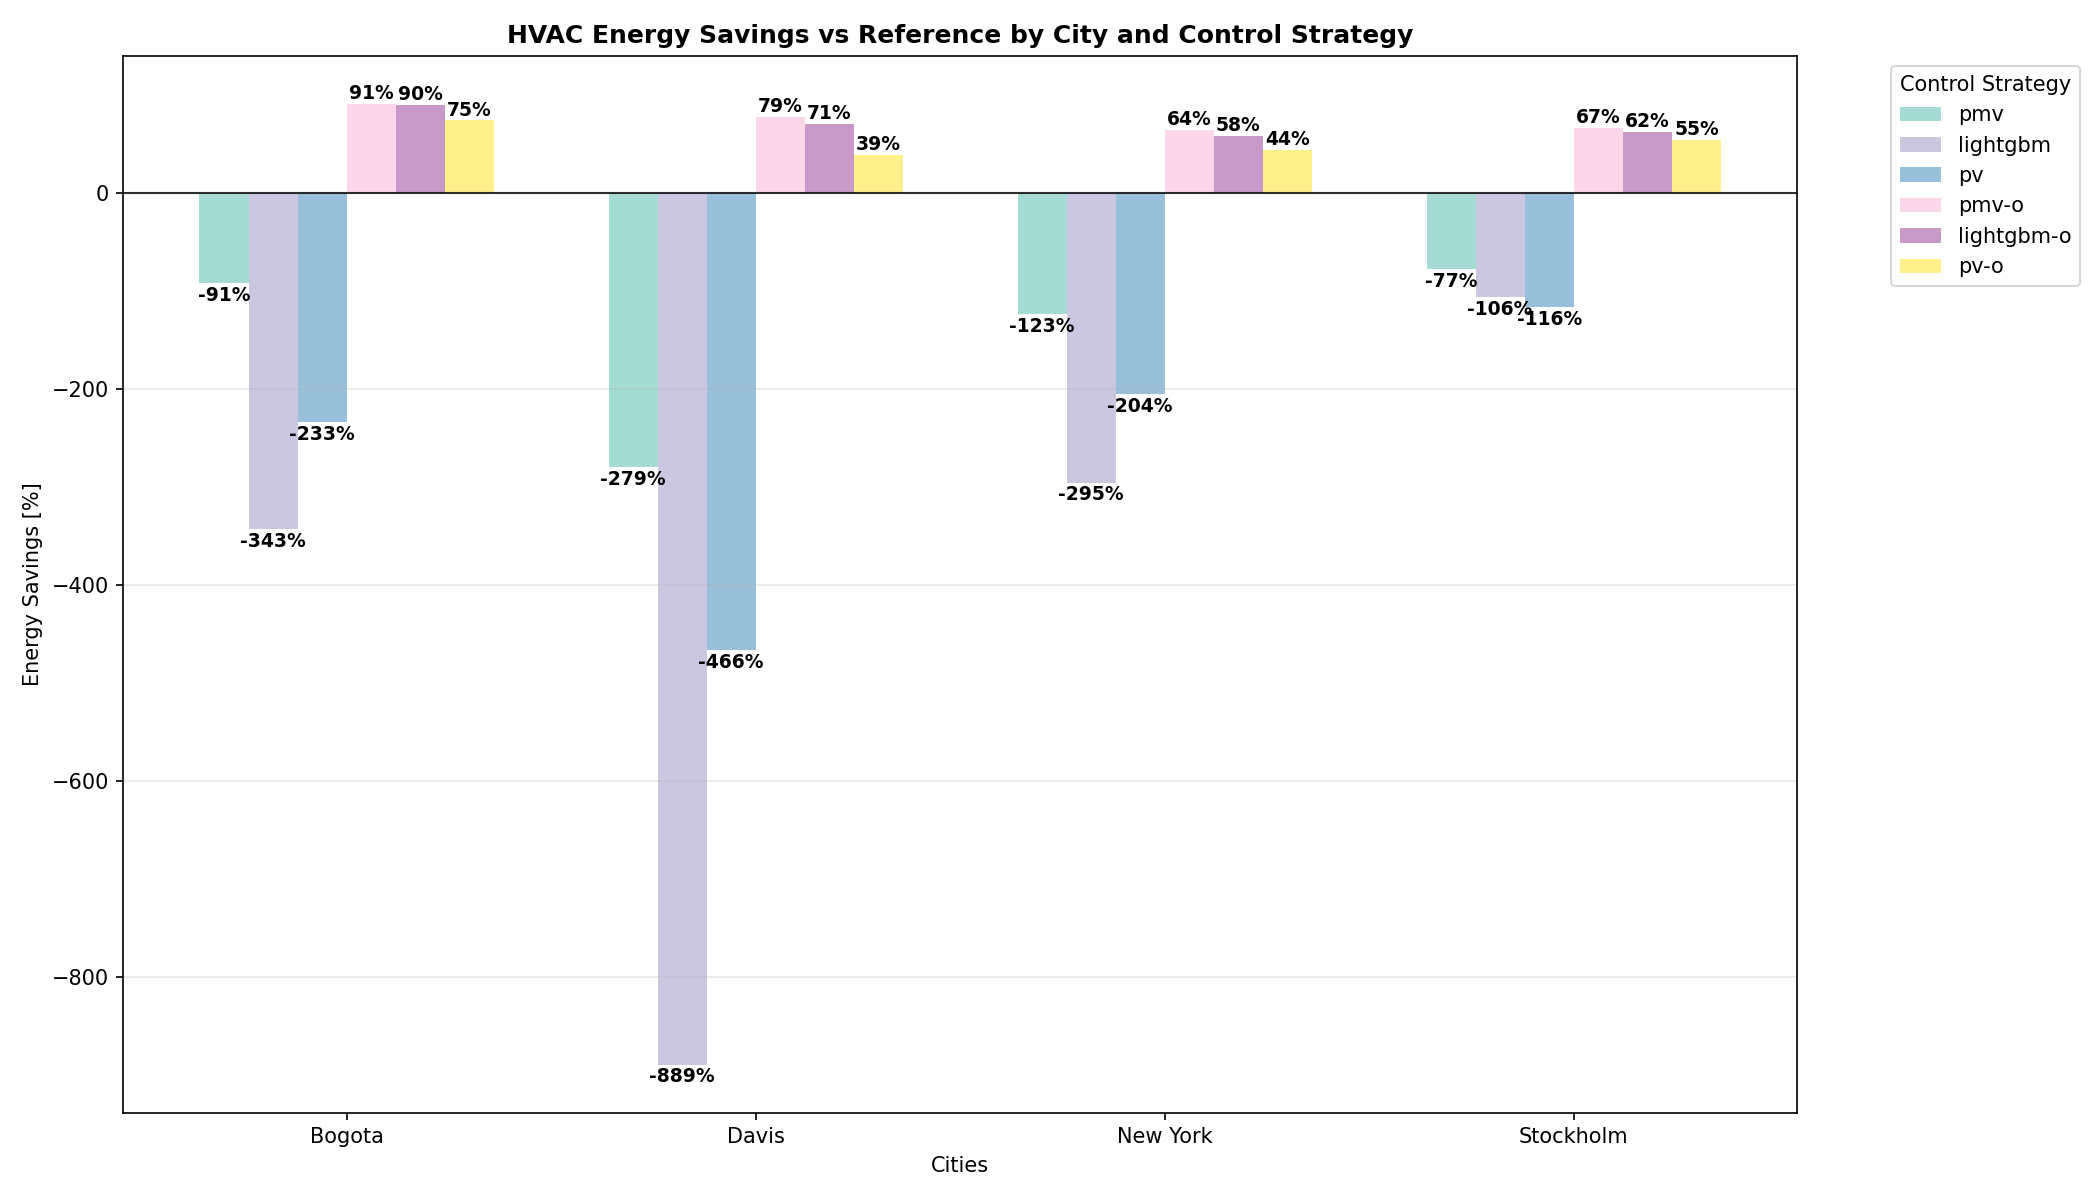
\includegraphics[width=\linewidth]{figs/savings_r.png}
    \caption{Total HVAC energy savings (\%) relative to \texttt{reference} across four cities. Grid‐search variants (\texttt{pmv-o}, \texttt{lightgbm-o}, \texttt{pv-o}) yield 62\%–90\% savings; unoptimized modes incur large negative savings due to actuator clipping.}
    \label{fig:hvac_savings}
\end{figure}


\subsubsection{Performance Hierarchy and Climate Consistency Analysis}
\label{sec:performance_hierarchy}
Having established the performance metrics, we now examine how these rankings remain consistent across diverse climates. 
As shown in Figure~\ref{fig:energy_ranking}, annual energy consumption (MJ/m²) for each control mode in Bogota, Davis‐Monthan, New York, and Stockholm (1 = most efficient) are plotted and ranked accordingly. Across all four climates, the optimized grid‐search variants (\texttt{pv-o}, \texttt{pmv-o}, \texttt{lightgbm-o}) occupy the top three positions, with \texttt{pv-o} and \texttt{pmv-o} typically tied for first or second. The baseline \texttt{reference} control consistently falls in the middle (rank 4), while the unoptimized “pure” modes (\texttt{pmv}, \texttt{pv}, \texttt{lightgbm}) occupy ranks 5–7, reflecting their inability to avoid actuator saturation.

While the previous section showed absolute performance differences, here we observe that climate-specific nuances appear primarily among the mid-rank and bottom modes, with top performers maintaining their advantage regardless of location. In Bogota and New York, \texttt{lightgbm-o} edges out \texttt{pmv-o} by a small margin, whereas in Davis‐Monthan and Stockholm, \texttt{pmv-o} ties or slightly outperforms \texttt{pv-o}. Among the unoptimized controllers, \texttt{pmv} often ranks lower in cold climates (Stockholm) but improves modestly in mixed or hot climates (Bogota, Davis‐Monthan). Similarly, \texttt{lightgbm} and \texttt{pv} without grid optimization display high variability—\texttt{lightgbm} fares better in New York but poorly in Davis‐Monthan, while \texttt{pv} consistently remains mid‐tier. Overall, the grid‐search optimization engenders both superior and more climate‐robust performance, demonstrating that a properly tuned analytical or ML‐based method consistently outperforms unoptimized strategies across diverse thermal conditions.


\subsubsection{Actuator Saturation Analysis}
\label{sec:actuator_saturation_results}
Our co-simulation methodology enables direct observation of actuator saturation behavior—a critical deployment challenge that pure comfort prediction research often overlooks. This phenomenon occurs when a controller's requested heating setpoint falls below the hard minimum ($12\,^\circ\mathrm{C}$) or its requested cooling setpoint exceeds the hard maximum ($30\,^\circ\mathrm{C}$). 
EnergyPlus (via Sinergym) then clips the setpoint to that boundary; further commands in the same direction have no effect. Table~\ref{tab:saturation_rates} demonstrates our framework's capability to quantify this saturation behavior, reporting the percentage of occupied hours during which each controller was clipped to 12 $\degree C$ or 30 $\degree C$ under both original and boundary-optimized implementations.

\begin{table}[!]
  \centering
  \caption{Percentage of occupied hours clipped to actuator bounds, before vs.\ after boundary optimization.}
  \label{tab:saturation_rates}
  \resizebox{\textwidth}{!}{
  \begin{tabular}{l|rrrrrr}
    \toprule
    \multirow{2}{*}{Controller Mode} & \multicolumn{3}{c}{Before} & \multicolumn{3}{c}{After} \\
    \cmidrule(lr){2-4} \cmidrule(lr){5-7}
    & \% @ 12~$^\circ$C & \% @ 30~$^\circ$C & \% Total Clipped
    & \% @ 12~$^\circ$C & \% @ 30~$^\circ$C & \% Total Clipped \\
    \midrule
    reference              & $0.00\%$ & $2.84\%$ & $2.84\%$ & $0.00\%$ & $2.85\%$ & $2.85\%$ \\
    PMV (pure)             & $0.00\%$ & $13.99\%$ & $13.99\%$ & $0.00\%$ & $0.10\%$ & $0.10\%$ \\
    LightGBM (pure)        & $4.52\%$ & $7.95\%$ & $7.95\%$ & $0.00\%$ & $4.52\%$ & $4.52\%$ \\
    PV (pure)              & $0.00\%$ & $0.39\%$ & $0.39\%$ & $0.00\%$ & $0.12\%$ & $0.12\%$ \\
    PMV-o (grid-search)    & $0.02\%$ & $66.95\%$ & $66.95\%$ & $0.00\%$ & $32.70\%$ & $32.70\%$ \\
    LightGBM-o (grid-search)& $0.00\%$ & $73.82\%$ & $73.82\%$ & $0.00\%$ & $32.70\%$ & $32.70\%$ \\
    PV-o (grid-search)     & $0.14\%$ & $67.76\%$ & $67.76\%$ & $0.00\%$ & $33.45\%$ & $33.45\%$ \\
    \bottomrule
  \end{tabular}
  }
\end{table}

Examining results from Table~\ref{tab:saturation_rates}, we could quickly come to the following key observations:
\begin{itemize}
  \item \textbf{Heating‐side saturation is eliminated after boundary optimization.} All controllers show $0.00\%$ clipped at $12\,^\circ\mathrm{C}$ in the ``After'' columns, confirming that the $\pm2\,^\circ\mathrm{C}$ grid around the interior reset prevents any candidate from falling below $12\,^\circ\mathrm{C}$.  
  \item \textbf{Cooling‐side saturation remains substantial.}  Even after boundary optimization, PMV‐o, LightGBM‐o, and PV‐o clip at $30\,^\circ\mathrm{C}$ approximately one‐third of occupied hours (32.70–33.45\%). This indicates that under hot conditions, all $\Delta T$ candidates eventually hit the hard ceiling, and the controller remains pinned until comfort can be restored by other means.  
  \item \textbf{Pure ML/PV controllers improve heating saturation but still clip on cooling.}  LightGBM (pure) goes from $4.52\%$ clipped at $12\,^\circ\mathrm{C}$ “Before” to $0.00\%$ “After,” but still clips at $30\,^\circ\mathrm{C}$ for $4.52\%$ of occupied hours. PV (pure) clips at $30\,^\circ\mathrm{C}$ for only $0.12\%$ “After,” down from $0.39\%$.  
  \item \textbf{Complete elimination of cooling saturation is unrealistic.}  In very hot climates or during periods of peak internal gains, any controller will at times demand a cooling setpoint below $30\,^\circ\mathrm{C}$. Because EnergyPlus enforces the $30\,^\circ\mathrm{C}$ ceiling, saturation at that limit is inevitable whenever comfort cannot be maintained otherwise.  
  \item \textbf{Value of the ``Before vs.\ After'' comparison.}  Reporting both sets of numbers reveals how boundary optimization transforms LightGBM (pure) and PV (pure) from pathological “always‐clipped” strategies into far more balanced approaches. For instance, LightGBM (pure) used to clip at $12\,^\circ\mathrm{C}$ for $4.52\%$ of hours, but LightGBM‐o never clips at $12\,^\circ\mathrm{C}$—instead, it only clips at $30\,^\circ\mathrm{C}$ for $32.70\%$ of hours, reflecting honest, interior comfort attempts.  
\end{itemize}
\noindent

These results have practical implication for future controller design, particularly when co-simulating with Machine-Learning-based control log. Any ML‐based or DL‐based control logic that does not explicitly account for these hard actuator bounds will likely exhibit high saturation rates and derive spurious energy‐comfort conclusions. Our boundary‐optimized grid search successfully removes “too‐cold” saturation entirely and reduces “too‐hot” saturation by roughly half. Further improvements may involve predictive models (e.g., Model Predictive Control), anti‐windup PIDs, or RL agents with an explicit clipping penalty to minimize residual saturation under extreme conditions.  

\subsection{Incorporation of Physiological Variables into Control Strategy}
\label{sec:tsk_results}
As outlined in Section~\ref{sec:pv_tsk_control}, two $T_{skin}$ incorporated control strategies based on boundary-optimized PINN-VAE strategy are further applied to the simulation experiments with the results shown in Table~\ref{tab:pv_tsk_results}. \texttt{pv-tsk-strict} strategy demonstrates a notable improvement in comfort evaluation (15.10\% on average) compared to \texttt{pv-o}, accompanied by a slight increase in energy consumption (1.97\% on average) while the \texttt{pv-tsk-loose} mode shows negligible differences.

\begin{table}[htbp]
\begin{center}
\small
\caption{Percentage Change in EUI and Uncomfort Hour (Simple ASHRAE 55-2004) for $T_{skin}$-involved Strategies Compared to \texttt{pv-o}}
\label{tab:pv_tsk_results}
\vspace{0.5em}
\setlength{\tabcolsep}{6pt} % Adjust spacing between columns
\begin{tabular}{lcc|cc}
\toprule
\makecell[l]{City/\\Site} 
& \multicolumn{2}{c|}{pv-tsk-strict} 
& \multicolumn{2}{c}{pv-tsk-loose} \\
\cmidrule(lr){2-3} \cmidrule(lr){4-5}
& EUI(\%) & Uncomfort Hour(\%) & EUI(\%) & Uncomfort Hour(\%) \\
\midrule
Bogota        & $1.90$ & $-11.83$ & $0.10$ & $-0.20$ \\
Stockholm     & $0.85$ & $-18.36$ & $-0.71$ & $1.33$ \\
Davis-Monthan & $2.30$ & $-11.65$ & $0.10$ & $0.04$  \\
New York      & $2.85$ & $-18.57$ & $0.14$ & $0.08$  \\
\midrule
Average       & $1.97$ & $-15.10$ & $-0.09$ & $0.32$ \\
\bottomrule
\end{tabular}
\vspace{0.5em} \\
\footnotesize
\textit{Note:} Negative values signify a decrease in EUI (energy savings) and uncomfort hour (comfort improvement).
\end{center}
\end{table}

We also investigated under what circumstances does the $T_{skin}$ exert more significant impact on regulating intensity. It is observed that, under conditions where setpoint adjustments are made and the $T_{skin}$ comfort requirement is not satisfied, the air temperature tends to be notably higher than average, and is particularly tightly clustered in cities with a wider range of air temperature, such as Stockholm and New York (Figure~\ref{fig:tsk_ta_distribution}), which is in line with some research \cite{mekjavicPerceptionThermalComfort2021} suggesting that the $T_{skin}$ is more sensitive in heating process and therefore more likely to deviate from comfort range. The finding indicates higher effectiveness of incorporating $T_{skin}$ in thermal regulation under hot conditions.

\begin{figure}[htbp]
    \centering
    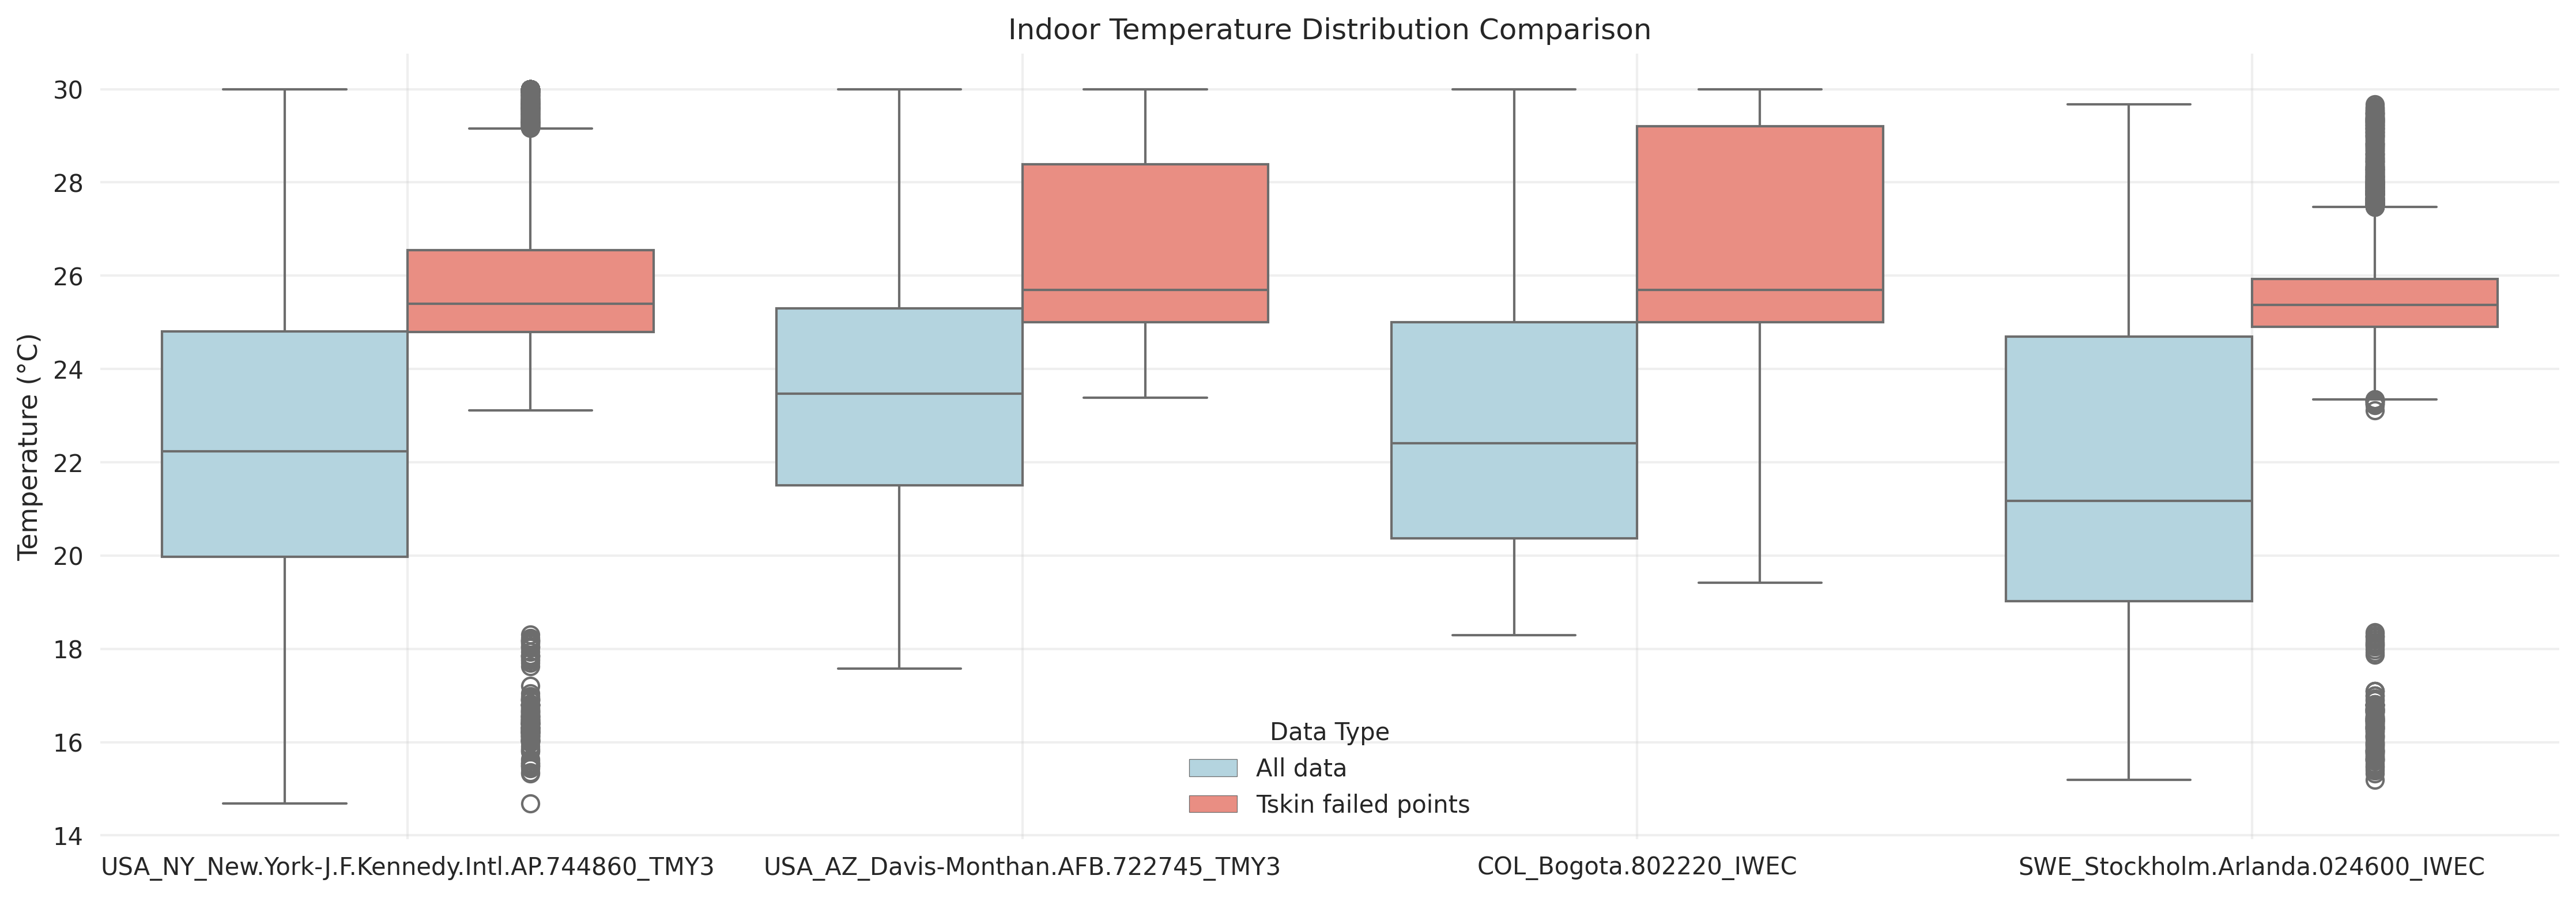
\includegraphics[width=0.75\linewidth]{figs/temp_distribution_comparison.png}
    \caption{Comparison of the air temperature distribution across all data points and the subset of instances where the $T_{skin}$ condition was not met with \texttt{pv-tsk-strict} mode}
    \label{fig:tsk_ta_distribution}
\end{figure}

Incorporating physiological metrics such as $T_{skin}$ into HVAC control logic significantly enhanced occupant comfort with minimal additional energy consumption. This result emphasizes the promising potential of physiology-informed control strategies to transform conventional building management approaches.



\subsection{Robustness Under Stochastic Weather Conditions}
The use of stochastic weather perturbations throughout our simulations provides inherent validation of our findings' statistical robustness. Despite random variations of $\pm$2.5$^\circ$C (1$\sigma$) applied to temperature readings at each 15-minute timestep—equivalent to sensor uncertainty and microclimate variations in real buildings—the performance hierarchy remains remarkably stable:
\begin{itemize}
    \item Grid-search optimized variants (pmv-o, lightgbm-o, pv-o) consistently rank in the top three positions across all climates
    \item Energy savings percentages show low variance: optimized PMV achieves 15-18.5\% savings with less than $\pm$2\% variation across weather realizations
    \item Comfort metrics remain stable: median PMV stays within $\pm$0.1 of target despite weather perturbations
\end{itemize}

This stability under stochastic conditions demonstrates that our findings are not artifacts of specific weather patterns but represent fundamental differences in control strategy effectiveness. The consistent performance gaps between optimized and naive controllers across thousands of unique weather realizations provide strong statistical evidence for our conclusions without requiring extensive Monte Carlo studies.

\section{Limitations and Future Work}

\subsection{Limitations}

\paragraph{Scope of Physiological Modeling:} The current implementation relies on Gagge’s two-node model to constrain physiological variables (core and skin temperature, skin wettedness). While widely used, this model simplifies thermal regulation and may not fully capture inter-individual variability or responses under extreme thermal conditions, physical exertion, or transient exposures.

\paragraph{Soft Constraints and Lack of Hard Guarantees:} The physiological constraints are enforced via soft penalties, which guide but do not guarantee adherence to biophysical bounds. In rare cases, especially under high imputation uncertainty or data sparsity, the model may still yield borderline physiological outputs that would not be biologically plausible under strict energy balance.

\paragraph{Dataset Bias and Underrepresented Populations:} Despite combining two large-scale datasets, certain groups—such as older adults, children, or individuals in tropical and arid climates—remain underrepresented. As a result, predictions for these populations may not generalize without additional targeted data.

\paragraph{Reliance on MAR Assumption:} While statistical tests and data context support the Missing At Random (MAR) assumption, any unobserved dependencies influencing missingness (i.e., potential MNAR characteristics) could theoretically affect imputation accuracy. However, VAE-based methods are generally considered robust under MAR, which we established as the most plausible scenario.

\paragraph{Operational Feasibility for Real-Time Applications:} While model interpretability and prediction quality are improved, the added complexity of latent-variable inference and physiology-based losses increases training and inference time. This may limit near-term deployment in embedded or low-latency building control systems without further optimization.


\subsection{Future Work}
\noindent We therefore believe there are at least the following possible directions of future work for PINN-VAE and its variants for thermal sensation:
\paragraph{Joint Optimization of Comfort and Physiology:} Given that PINN-VAE outputs not only thermal sensation but also skin and core temperatures, future work could explore control algorithms that co-optimize predicted thermal comfort and physiological deviation from neutral. This opens new opportunities for occupant-aware HVAC strategies that balance subjective sensation with biophysical safety margins.

\paragraph{Integration of Wearable and Streaming Data:} Future deployments may leverage wearable sensors or IoT devices to dynamically update personal physiological inputs (e.g., real-time skin temperature or heart rate), enabling the PPI interface to adapt to intra-occupant variation or temporal changes such as illness, stress, or activity level.

\paragraph{Architectural Simplification and Model Compression:} To support deployment in building systems with limited computational capacity, model compression techniques such as pruning, quantization, or teacher-student distillation could be applied to PINN-VAE. These techniques would aim to preserve interpretability while reducing inference time and memory usage.

\paragraph{Alternative Physiological and Comfort Models:} The current architecture could be extended to accommodate other biothermal models (e.g., Stolwijk\cite{Stolwijk1971} or multi-segment models like JOS3\cite{Takahashi2002JOS}) or adaptive comfort formulations that better reflect behavioral and cultural variability. Comparative evaluation would help assess trade-offs in complexity and predictive value.

\paragraph{Field Validation in Operational Settings:} Beyond retrospective evaluation, a key next step is validating PINN-VAE in real-world building environments, comparing predictions to occupant feedback and observed control behavior. This will test not only accuracy but also acceptance and integration into control workflows.

\section{Conclusions}
This study introduced a physiology-informed neural framework (PINN-VAE) that jointly addresses two core challenges in thermal comfort modeling: (i) imputing missing values in large observational datasets and (ii) improving predictive performance while preserving physiological interpretability. By embedding soft physiological constraints into a variational autoencoder pipeline and leveraging both tabular and personal-profile inputs, our model successfully balances the flexibility of data-driven imputation with the structure of thermoregulatory realism.

We demonstrate that PINN-VAE achieves comparable or superior performance to traditional state-of-the-art models, particularly near the thermal neutral zone, where directional prediction errors are often most critical for occupant-centric applications. The inclusion of intermediate physiological outputs—core and skin temperatures—not only constrains unrealistic predictions but also offers interpretability advantages unavailable in tree-based or purely statistical models.

Furthermore, the availability of intermediate physiological outputs ($\hat{T}_{\text{core}}, \hat{T}_{\text{skin}}, \hat{w}$) offers enhanced interpretability; beyond predicting sensation, monitoring these variables could enable systems to infer underlying physiological states, potentially allowing for more proactive or health-aware environmental control strategies that anticipate discomfort or thermal stress.

Beyond thermal comfort, the PINN-VAE architecture offers a generalizable framework for combining latent-variable learning with physics-informed constraints. Its use could extend to domains such as biomechanics, energy metabolism modeling, or any setting where tabular physiological data are incomplete yet governed by known physical relationships.

The Personalized Physiology Interface (PPI) further strengthens this framework by enabling the use of raw demographic variables (e.g., age, height, gender, weight) without degrading predictive performance. In doing so, the model preserves important physiological signal diversity without needing population-wide feature averaging or scaling.

Compared to baseline LightGBM and unconstrained VAE architectures, our framework shows a measurable reduction in neutral-zone RMSE and direction-penalty asymmetry, reinforcing the hypothesis that physiology-informed modeling improves both accuracy and robustness. Overall, PINN-VAE offers a promising and interpretable path forward for occupant-aware control, particularly in systems where physiological realism and explainability are essential for deployment.



\section*{Data and Code Availability}
The code developed for the PINN-VAE model and the analysis presented in this paper is available on GitHub at [URL Currently Private] The final imputed dataset, generated using the best-performing model fold as described in Section~\ref{sec:PINN_VAE_Arch}, is available at request (currently sitting on private repository on github). The original ASHRAE Global Thermal Comfort Database II and Chinese Thermal Comfort Datasets are publicly available from their respective sources cited in the text.
%% Add \usepackage{lineno} before \begin{document} and uncomment 
%% following line to enable line numbers
%% \linenumbers

%% main text
%%
% \section{Introduction}
%% Use \section commands to start a section
% \section{Example Section}
% \label{sec1}
% %% Labels are used to cross-reference an item using \ref command.

% Section text. See Subsection \ref{subsec1}.

% %% Use \subsection commands to start a subsection.
% % \subsection{Example Subsection}
% \label{subsec1}

% Subsection text.

% %% Use \subsubsection, \paragraph, \subparagraph commands to 
% %% start 3rd, 4th and 5th level sections.
% %% Refer following link for more details.
% %% https://en.wikibooks.org/wiki/LaTeX/Document_Structure#Sectioning_commands

% \subsubsection{Mathematics}
% %% Inline mathematics is tagged between $ symbols.
% This is an example for the symbol $\alpha$ tagged as inline mathematics.

% %% Displayed equations can be tagged using various environments. 
% %% Single line equations can be tagged using the equation environment.
% \begin{equation}
% f(x) = (x+a)(x+b)
% \end{equation}

% %% Unnumbered equations are tagged using starred versions of the environment.
% %% amsmath package needs to be loaded for the starred version of equation environment.
% \begin{equation*}
% f(x) = (x+a)(x+b)
% \end{equation*}

% %% align or eqnarray environments can be used for multi line equations.
% %% & is used to mark alignment points in equations.
% %% \\ is used to end a row in a multiline equation.
% \begin{align}
%  f(x) &= (x+a)(x+b) \\
%       &= x^2 + (a+b)x + ab
% \end{align}

% \begin{eqnarray}
%  f(x) &=& (x+a)(x+b) \nonumber\\ %% If equation numbering is not needed for a row use \nonumber.
%       &=& x^2 + (a+b)x + ab
% \end{eqnarray}

% %% Unnumbered versions of align and eqnarray
% \begin{align*}
%  f(x) &= (x+a)(x+b) \\
%       &= x^2 + (a+b)x + ab
% \end{align*}

% \begin{eqnarray*}
%  f(x)&=& (x+a)(x+b) \\
%      &=& x^2 + (a+b)x + ab
% \end{eqnarray*}

% %% Refer following link for more details.
% %% https://en.wikibooks.org/wiki/LaTeX/Mathematics
% %% https://en.wikibooks.org/wiki/LaTeX/Advanced_Mathematics

% %% Use a table environment to create tables.
% %% Refer following link for more details.
% %% https://en.wikibooks.org/wiki/LaTeX/Tables
% \begin{table}[t]%% placement specifier
% %% Use tabular environment to tag the tabular data.
% %% https://en.wikibooks.org/wiki/LaTeX/Tables#The_tabular_environment
% \centering%% For centre alignment of tabular.
% \begin{tabular}{l c r}%% Table column specifiers
% %% Tabular cells are separated by &
%   1 & 2 & 3 \\ %% A tabular row ends with \\
%   4 & 5 & 6 \\
%   7 & 8 & 9 \\
% \end{tabular}
% %% Use \caption command for table caption and label.
% \caption{Table Caption}\label{fig1}
% \end{table}


% %% Use figure environment to create figures
% %% Refer following link for more details.
% %% https://en.wikibooks.org/wiki/LaTeX/Floats,_Figures_and_Captions
% \begin{figure}[t]%% placement specifier
% %% Use \includegraphics command to insert graphic files. Place graphics files in 
% %% working directory.
% \centering%% For centre alignment of image.
% \includegraphics{example-image-a}
% %% Use \caption command for figure caption and label.
% \caption{Figure Caption}\label{fig1}
% %% https://en.wikibooks.org/wiki/LaTeX/Importing_Graphics#Importing_external_graphics
% \end{figure}


% %% The Appendices part is started with the command \appendix;
% %% appendix sections are then done as normal sections
\appendix
\section{Appendix}
\subsection{Acronyms and Glossary of Terms}

\printglossary[type=\acronymtype, title=Acronyms]
\printglossary[title=Glossary of Terms]

\subsection{Data Alignment Table}\label{sec:alignment}
To provide better context of how the data alignment is performed across different columns and their correspoding fields of interests, we have included the table we used to map accordingly as showon in Table~\ref{tab:table-map}.

\begin{table}[h!]
  \centering
  \resizebox{\textwidth}{!}{%
    \begin{tabular}{|l|l|l|l|}
      \hline
      \textbf{Unified Column} & \textbf{Chinese (Set 1) Column} & \textbf{ASHRAE (Set 2) Column} & \textbf{Notes} \\ \hline
      timestamp                      & date\_clean                     & timestamp            & $\surd$ \\ \hline
      contributor                    & a3.data contributor            & contributor          & $\surd$ \\ \hline
      season                         & a4.season                      & season               & Chinese has transition season. \\ \hline
      city                           & a5.city                        & city                 & $\surd$ \\ \hline
      climate\_zone                  & a6.climate zone                & climate              & Totally different categorization methods. \\ \hline
      building\_type                 & b1.building type               & building\_type       & Categories different. \\ \hline
      gender                         & c1.sex                         & gender               & $\surd$ \\ \hline
      age                            & c2.age                         & age                  & $\surd$ \\ \hline
      height\_cm                     & c3.height(cm)                & ht                   & $\surd$ \\ \hline
      weight\_kg                     & c4.weight(kg)                & wt                   & $\surd$ \\ \hline
      thermal\_sensation             & d1.tsv                         & thermal\_sensation   & $\surd$ \\ \hline
      thermal\_comfort               & d2.tcv                         & thermal\_comfort     & Different numerical evaluation criteria. \\ \hline 
      thermal\_acceptability         & d3.tav                         & thermal\_acceptability & Different numerical evaluation criteria. \\ \hline
      clothing\_insulation           & d5.clothing insulation (clo)   & clo                  & $\surd$ \\ \hline
      metabolic\_rate                & d6.metabolic rate (met)        & met                  & $\surd$ \\ \hline
      mean\_radiant\_temperature      & f2.mean radiant temperature ($\degree C$) & tr                 & Calculated MRT\\ \hline
      pmv\_ce                       & f4.pmv                         & pmv\_ce              & $\surd$ \\ \hline
      ppd\_ce                       & f5.ppd                         & ppd\_ce              & $\surd$ \\ \hline
      ta\_l                         & e1.indoor air temperature ($\degree C$)   & ta\_l                & air temperature @0.1 m \\ \hline
      ta                            & e1.indoor air temperature ($\degree C$).1 & ta                   & air temperature @0.6 m \\ \hline
      ta\_h                         & e1.indoor air temperature ($\degree C$).2 & ta\_h                & air temperature @1.1 m \\ \hline
      vel\_l                        & e3.indoor air velocity (m/s)    & vel\_l               & air velocity @0.1 m  (m/s, fpm) \\ \hline
      vel                           & e3.indoor air velocity (m/s).1  & vel                  & air velocity @0.6 m  (m/s, fpm) \\ \hline
      vel\_h                        & e3.indoor air velocity (m/s).2  & vel\_h               & air velocity @1.1 m  (m/s, fpm) \\ \hline
      rh                            & e2.indoor relative humidity (\%) & rh                 & relative humidity not available at different heights.\\ \hline
      tg\_l                        & e4.globe temperature ($\degree C$)        & tg\_l               & Globe temperature at 0.1 m \\ \hline
      tg                           & e4.globe temperature ($\degree C$).1      & tg                  & Globe temperature at 0.6 m \\ \hline
      tg\_h                        & e4.globe temperature ($\degree C$).2      & tg\_h               & Globe temperature at 1.1 m \\ \hline
      to                           & f1.operative temperature ($\degree C$)    & top                 & $\surd$ \\ \hline
      year                         & year                           & year                & $\surd$ \\ \hline
      country                      & country                        & country             & $\surd$ \\ \hline
      coolingsys                   & b4.building operation mode     & cooling\_type       & Inconsistent definition. \\ \hline
      latitude                     & latitude                       & lat                 & generated with geopy from city info.\\ \hline
      longitude                    & longitude                      & lon                 & generated with geopy from city info. \\ \hline
      ta\_out & g3.Monthly Mean Outdoor Temperature($\degree C$)    & ta\_out             & $\surd$ \\ \hline
      \end{tabular}}
  \caption{Database alignment mapping between ASHRAE II and Chinese Thermal Comfort Databases}
  \label{tab:table-map}
\end{table}

\subsection{Frozen PPI Weights}
While the Personalized Physiology Interface (PPI) header was introduced to leverage individual demographic data, its impact on overall performance (model \texttt{pvp\_pen}) yielded only marginal improvements compared to the standard PINN-VAE (\texttt{pv\_pen}), as seen in Table~\ref{tab:performance_updated} and Figure 6. Although the improvement was consistent, it was not deemed sufficiently notable within the scope of this preliminary exploration to warrant extensive discussion. Further investigation is needed to fully understand how to maximize the benefit of such personalization. Future work could explore enhancing the PPI by integrating dynamic data, such as real-time physiological measurements from wearable sensors, potentially unlocking more significant performance gains and adaptability.

%Add one more table and we're done.

Nevertheless, we were able to freeze the final PPI weights across our proposed header addition to the PINN-VAE framework, notably the PPI-ANALYTIC Model as outlined in Figure~\ref{fig:workflow}. As was discussed inside the results and discussion section of this paper, its improvement upon the PINN-VAE model was clear yet minimal. Hence this header architecture was not pursued any further beyond the following table with weights frozen.


% % \section{Example Appendix Section}
% % \label{app1}

% % Appendix text.

% % %% For citations use: 
% % %%       \citet{<label>} ==> Lamport (1994)
% % %%       \citep{<label>} ==> (Lamport, 1994)
% % %%
% % Example citation, See \citet{lamport94}.

% % %% If you have bib database file and want bibtex to generate the
% % %% bibitems, please use
% % %%
% % %%  \bibliographystyle{elsarticle-harv} 
% % %%  \bibliography{<your bibdatabase>}

% % %% else use the following coding to input the bibitems directly in the
% % %% TeX file.

% % %% Refer following link for more details about bibliography and citations.
% % %% https://en.wikibooks.org/wiki/LaTeX/Bibliography_Management

% % \begin{thebibliography}{00}

% % %% For authoryear reference style
% % %% \bibitem[Author(year)]{label}
% % %% Text of bibliographic item

% % \bibitem[Lamport(1994)]{lamport94}
% %   Leslie Lamport,
% %   \textit{\LaTeX: a document preparation system},
% %   Addison Wesley, Massachusetts,
% %   2nd edition,
% %   1994.

% % \end{thebibliography}
\bibliographystyle{IEEEtran} % or another style as per journal requirements
\bibliography{cas-refs}

\end{document}

\endinput
%%
%% End of file `elsarticle-template-harv.tex'.


